%% Adaptado a partir de :
%%    abtex2-modelo-trabalho-academico.tex, v-1.9.2 laurocesar
%% para ser um modelo para os trabalhos no IFSP-SPO

\documentclass[
    % -- opções da classe memoir --
    12pt,               % tamanho da fonte
    openright,          % capítulos começam em pág ímpar (insere página vazia caso preciso)
    %twoside,            % para impressão em verso e anverso. Oposto a oneside
    oneside,
    a4paper,            % tamanho do papel. 
    % -- opções da classe abntex2 --
    %chapter=TITLE,     % títulos de capítulos convertidos em letras maiúsculas
    %section=TITLE,     % títulos de seções convertidos em letras maiúsculas
    %subsection=TITLE,  % títulos de subseções convertidos em letras maiúsculas
    %subsubsection=TITLE,% títulos de subsubseções convertidos em letras maiúsculas
    % para pacote url reconhecer hifens como separador
    hyphens,
%    paginasA3,  % indica que vai utilizar paginas em A3 
    % Opções que não devem ser utilizadas na versão final do documento
    draft,              % para compilar mais rápido, remover na versão final
    MODELO,             % indica que é um documento modelo então precisa dos geradores de texto
    TODO,               % indica que deve apresentar lista de pendencias 
    % -- opções do pacote babel --
    english,            % idioma adicional para hifenização
    brazil           % o último idioma é o principal do documento
    ]{ifsp-spo-inf-cpti} % ajustar de acordo com o modelo desejado para o curso

% ---
% Pacotes básicos 
% ---
%\usepackage[utf8]{inputenc}     % Codificacao do documento (conversão automática dos acentos)
% ---

%\usepackage{style}
        


% --- 
% CONFIGURAÇÕES DE PACOTES ADICIONAIS UTEIS
% --- 
\usepackage{pdfpages}			% para incluir arquivos pdf no documento


% ---
% Informações de dados para CAPA e FOLHA DE ROSTO
% ---
\titulo{TÍTULO DO TRABALHO}
\autor{AUTOR DO TRABALHO}

\preambulo{Modelo canônico de trabalho monográfico acadêmico em conformidade com
as normas ABNT apresentado à comunidade de usuários \LaTeX.}

% Para versões intermediarias utilizar a data
% Para versão final de monografia utilizar o ano do depósito
\data{DATA DO TRABALHO}

% Definir o que for necessário e comentar o que não for necessário
% Utilizar o Nome Completo
\orientador{ORIENTADOR}
\coorientador{COORIENTADOR}

% ---


% informações do PDF
\makeatletter
\hypersetup{
        %pagebackref=true,
        pdftitle={\@title}, 
        pdfauthor={\@author},
        pdfsubject={\imprimirpreambulo},
        pdfcreator={LaTeX with abnTeX2 using IFSP model},
        pdfkeywords={abnt}{latex}{abntex}{abntex2}{IFSP}{\ifspprefixo}{trabalho acadêmico}, 
        colorlinks=true,            % false: boxed links; true: colored links
        linkcolor=blue,             % color of internal links
        citecolor=blue,             % color of links to bibliography
        filecolor=magenta,              % color of file links
        urlcolor=blue,
        bookmarksdepth=4
}
\makeatother
% --- 


% ----
% Início do documento
% ----
\begin{document}


% Retira espaço extra obsoleto entre as frases.
\frenchspacing 

%somente para o exemplo, fica primeiro
%\input{00-teste}
\newcommand{\urlmodelosimples}{https://www.sharelatex.com/project/58a3a66af9bb74023ba1bd56}

\newcommand{\urlmodelo}{\url{\urlmodelosimples}}




\newpage


% -- lista de pendencias gerada pelo todonotes
% -- altere opções do usepackage para remover na versão final....
\listoftodos
\todo[inline]{remover lista de todo da versão final...}
\newpage

% ----------------------------------------------------------
% ELEMENTOS PRÉ-TEXTUAIS
% ----------------------------------------------------------
\pretextual

% ---
% Capa
% ---
\imprimircapa

\newcounter{todocounter}
\newcommand{\todonum}[2][]
{\stepcounter{todocounter}\todo[#1]{\thetodocounter: #2}}


\todonum[inline]{ajustar titulo do trabalho}
\todonum[inline]{ajustar autor}
\todonum[inline]{ajustar data}
\todonum[inline]{ajustar preambulo}
\todonum[inline]{ajustar curso}
\todonum[inline]{ajustar disciplina}
\todonum[inline]{ajustar departamento}
\todonum[inline]{ajustar orientador/coorientador/professor(es)}
% ---

% ---
% Folha de rosto
% (o * indica que haverá a ficha bibliográfica)
% ---
\imprimirfolhaderosto
%\imprimirfolhaderosto*
% ---

% Quando registrado na biblioteca
%\input{pre-fichacatalografica}

%Caso necessário
%\input{pre-errata}

%Obrigatório para trabalhos com bancas oficiais
%\input{pre-aprovacao}

% ---- opcionais 
% ---
% Dedicatória
% ---
\begin{dedicatoria}
   \vspace*{\fill}
   \centering
   \noindent
   \textit{ Este trabalho é dedicado às crianças adultas que,\\
   quando pequenas, sonharam em se tornar cientistas.} 

\todonum[inline]{colocar sua dedicatoria}
   
   \vspace*{\fill}
   

\end{dedicatoria}
% ---
% ---
% Agradecimentos
% ---
\begin{agradecimentos}
%\todonum[inline]{colocar seus agradecimentos}
Os principais agradecimentos são direcionados ao casal Dario e Isis França, irmão e cunhada, respectivamente, da Product Owner Tayna França, que foram a base e motivação para a criação do projeto diversaGente e que foram de enorme valor para a compreensão da realidade das pessoas neurodiversas e das que estão em volta delas.

Os agradecimentos especiais se direcionam aos professores José Braz de Araújo e Marcelo Tavares de Santana, que, durante todo o desenvolvimento do projeto, estiveram abertos a apoiar e aconselhar com o que fosse necessário, passando orientações e feedbacks de forma clara e direta.

Por fim, agradecimentos à todos que, de alguma forma, contribuíram para que o projeto fosse concluído.

\end{agradecimentos}
% ---
\input{pre-epigrafe}

% -- resumo obrigatório
% ---
% RESUMOS
% ---

% resumo em português
\setlength{\absparsep}{18pt} % ajusta o espaçamento dos parágrafos do resumo
\begin{resumo}
\todo[inline]{fazer o seu resumo, ele só é feito depois que o documento está terminado
\newline
\newline os itens em negrito estão aqui para ressaltar detalhes que devem ser seguidos, mas não se utiliza o negrito em um resumo}

 De acordo com a norma \citetitle{NBR6028:2003} (3.1-3.2) \index{NBR6028}, o resumo\index{resumo} deve ressaltar o contexto, o objetivo, o método, os resultados e as conclusões do documento (portanto deve ser escrito por ultimo). A ordem e a extensão destes itens dependem do tipo de resumo (informativo ou indicativo) e do  tratamento que cada item recebe no documento original. O resumo \textbf{deve ter um paragrafo único} e deve \textbf{ter entre 150 e 500 palavras para trabalhos acadêmicos ou entre 100 e 250 para artigos de periódicos}. O resumo deve ser  precedido da referência do documento, com exceção do resumo inserido no  próprio documento. (\ldots) As palavras-chave devem figurar logo abaixo do resumo, antecedidas da expressão \textbf{Palavras-chave}:, separadas entre si por ponto e finalizadas também por ponto.

 \textbf{Palavras-chaves}: latex. abntex. editoração de texto.
\end{resumo}

% resumo em inglês
\begin{resumo}[Abstract]
 \begin{otherlanguage*}{english}

   This is the english abstract.

\todo[inline]{fazer tradução do resumo, não utilizar tradução automática}

\todo[inline]{Cuidado com termos que só fazem sentido na língua portuguesa, o texto deve ser ajustado para fazer sentido aos leitores que não conhecem a língua portuguesa}

   \vspace{\onelineskip}

   \noindent 
   \textbf{Keywords}: latex. abntex. text editoration.
 \end{otherlanguage*}
\end{resumo}


% ---
% inserir lista de ilustrações
% ---
\pdfbookmark[0]{\listfigurename}{lof}
\listoffigures*
\cleardoublepage
% ---

% ---
% inserir lista de tabelas
% ---
\pdfbookmark[0]{\listtablename}{lot}
\listoftables*
\cleardoublepage
% ---

% ---
% inserir lista de quadros
% ---
\pdfbookmark[0]{\listofquadrosname}{loq}
\listofquadros*
\cleardoublepage
% ---

% ---
% inserir lista de abreviaturas e siglas
% ATENCAO o SHARELATEX/OVERLEAF GERA O GLOSSARIO SOMENTE UMA VEZ
% CASO SEJA FEITA ALGUMA ALTERAÇÃO NA LISTA DE SIGLAS É NECESSARIO UTILIZAR A OPÇÃO :
% "Clear Cached Files" DISPONIVEL NA VISUALIZAÇÃO DOS LOGS 
% ---
% https://www.sharelatex.com/learn/Glossaries


\ifdef{\printnoidxglossary}{
    \printnoidxglossary[type=\acronymtype,title=Lista de abreviaturas e siglas,style=siglas]
    \cleardoublepage
}{}


\input{pre-simbolos}
\todo[inline]{Remover lista de simbolos se não for necessário}


% ---
% inserir o sumario
% ---
\pdfbookmark[0]{\contentsname}{toc}
\tableofcontents*
\cleardoublepage
% ---


% ----------------------------------------------------------
% ELEMENTOS TEXTUAIS
% ----------------------------------------------------------
\textual


% ----------------------------------------------------------
% Introdução
% ----------------------------------------------------------
\chapter[Metodologia de gestão de projeto e desenvolvimento utilizadas. ]{Metodologia de gestão de projeto e desenvolvimento utilizadas.}

A metodologia que o grupo escolheu para ser usado é o Scrum. Primeiramente pelo fato de ser ágil e também por estarmos em um desenvolvimento de projeto no qual haverá necessidade de programar uma rede social e o Scrum atualmente é amplamente utilizado por equipes de desenvolvedores e também por ser a que o grupo está mais habituado a trabalhar.

Como estamos seguindo a metodologia ágil Scrum, existe uma “hierarquia” e responsabilidades para que o desenvolvimento seja o mais eficiente possível. Para a nossa equipe decidimos optar pelos cargos de Scrum Master, Product Owner e Desenvolvedores.

\begin{itemize}
    \item Scrum Master sendo o responsável para que a estrutura do Scrum seja seguida e realizada. Tira empecilhos de membros da equipe para que o desenvolvimento não seja comprometido, verifica a necessidade de adaptação do Scrum e obter um melhor fluxo de trabalho. O Gustavo Freitas ficou com a função de ser o Scrum Master do time.
    
    \item Tayna França Soza é a Product Owner (PO) da equipe e “representa os interesses de stakeholders (no sentido de agregar valor ao negócio), define funcionalidades do produto e faz a gestão do backlog, priorizando tarefas segundo métodos ágeis, como o Scrum.” (Equipe PM3, 2022)
    
    \item Desenvolvedores são os responsáveis de verificar como que as alterações propostas pelo PO vão ser feitas e se podem ser feitas, integrações, modelagem de banco de dados, programação de código do projeto, definir arquitetura e padronização de commits e documentação do código para que ele tenha uma manutenibilidade alta caso seja necessário manutenções futuras e colocar a aplicação em produção sem nenhum problema futura. Os responsáveis por essas funções são: Gabriel Ruiz, Grazielli Berti, João Bispo, Vinicius Soares e Viviane Queiroz.
    
\end{itemize}


% ---
% Capitulo de revisão de literatura
% ---
\chapter{Revisão da Literatura}


Neste tópico fazer um estudo e tirar observações mais a fundo a respeito da neurodiversidade. Relatar quando começou os estudos a respeito das pessoas neurodiversas e entender como foi o papel da sociedade no passado, no que nisso acarretou e as mudanças necessárias que surgiram para chegar nos dias de hoje. 
\section{Influência do termo}
As questões neurodiversas em toda sociedade sempre foi um assunto difícil de falar, principalmente porque no passado era tratado com "modelo de tragédia pessoal" \cite{oliver1990politics}. Dessa maneira, foi crescendo o indiferente e o inquestionável a  respeito das pessoas que sofrem algum tipo de neurodiversidade. Entretanto, com os estudos, os teóricos que estudavam a causa mais fundo diziam que esse modelo social estaria equivocado, pois se deixar que essa percepção percorra nossa sociedade não irá trazer as necessárias responsabilidades sociais que devemos atingir para evitar esses equívocos. 
Sendo assim, essa mudança de responsabilidade para o comportamento com as neurodiversidades promove o empoderamentos do indivíduo e sendo assim ele ganha espaço para ser olhado pela sociedade e respeitado por elas. 

\section{Virada de responsabilidades}
Um dos motivos que nos levou a trazer o tema da neurodiversidade para o nosso projeto final está na maneira que o assunto é tratado na sociedade. Há muitos tabus a serem derrubados. Se, por volta de 1960, ainda se culpavam os pais pela pelos seus filhos terem nascido com alguma neurodiversidade e, portanto, impossibilitava o surgimentos de movimentos que pudessem entender e ajudar os familiares,hoje temos algumas conquistas a serem celebradas como projetos de leis que protejam as pessoas neurodiversas graças aos estudos sobre deficiência nos anos 70 que desconstruiu um modelo de responsabilidade única para uma socialmente construída.\cite{ortega}
Todavia, o preconceito, falta de informação e suporte ainda estão presentes no convívio social e dessa maneira, trazer uma rede social focada para sanar dúvidas e compartilhar informações e serviços torna-se esse assunto vivo diante a sociedade.  

\section{Responsabilidade do Aplicativo}
Apontado no artigo de \cite{rios}, evidencia-se que no Brasil há um embate entre profissionais e pais a respeito do movimento neurodiverso, uma vez que a sociedade brasileira ainda está atrelada aos modelos ultrapassados lá da décadas de 1960. Dessa maneira, o diversaGente tem como objetivo tornar-se um ambiente de discussões e compartilhamento de informações sobre o assunto. 
Assim, o comprometimento na era digital que vivemos junto com a neurodiversidade nos remete ao compartilhamento de mais informações a respeito do assuntos com pessoas em diversos lugares, diversas famílias e culturas, pois em diversos artigos apresentam críticas a forma que os métodos atuais de tratamento são usados, uma vez que muitos tratamentos centram-se na deficiência e não na forma humana que deve ser tratado. \cite{machado} 



% Para facilitar a manutenção é sempre melhore criar um arquivo por capitulo, para exemplo isso não é necessário 
% Para facilitar a manutenção é sempre melhore criar um arquivo por capitulo, para exemplo isso não é necessário 

%---------------------------------------------------------------------------------------


% Para facilitar a manutenção é sempre melhore criar um arquivo por capitulo, para exemplo isso não é necessário 

%---------------------------------------------------------------------------------------
\chapter{Gestão do projeto}

A metodologia de gestão de projetos escolhida foi baseada no Scrum. Primeiramente pelo fato da metodologia prezar a independência de todos da equipe, pela rapidez, agilidade de agregar valor para o cliente e produto final e segundo pelos membros da equipe já se familializarem com o modelo, uma vez que todos praticam esse modelo em seus respectivos trabalhos. 

Como foi decidido pela metodologia ágil Scrum, existe uma “hierarquia” e responsabilidades para que o desenvolvimento seja o mais eficiente possível. Para a nossa equipe há os cargos de Scrum Master, Product Owner e Desenvolvedores.

\begin{itemize}
	\item Scrum Master sendo o responsável para que a estrutura do Scrum seja seguida e realizada. Tira empecilhos de membros da equipe para que o desenvolvimento não seja comprometido, verifica a necessidade de adaptação do Scrum e obter um melhor fluxo de trabalho. O Gustavo Freitas ficou com a função de ser o Scrum Master do time.
	
	\item Tayna França Soza é a Product Owner (PO) da equipe e “representa os interesses de stakeholders (no sentido de agregar valor ao negócio), define funcionalidades do produto e faz a gestão do backlog, priorizando tarefas segundo métodos ágeis, como o Scrum.” \cite{especificações_do_PO}
	
	\item Desenvolvedores são os responsáveis de verificar como que as alterações propostas pelo PO vão ser feitas e se podem ser feitas, integrações, modelagem de banco de dados, programação de código do projeto, definir arquitetura e padronização de commits e documentação do código para que ele tenha uma manutenibilidade alta caso seja necessário manutenções futuras e colocar a aplicação em produção sem nenhum problema futuro. Os responsáveis por essas funções são: Gabriel Ruiz, Grazielli Berti, João Bispo, Vinicius Soares e Viviane Queiroz.
	
\end{itemize}

Apesar de cada membro da equipe ter as suas funções muito bem estabelecidas como detalhado no \autoref{responsabilidade-integrantes} todos têm uma contribuição na construção do código da aplicação, sendo assim, mesmo que em menor quantidade, o Product Owner e Scrum Master precisam contribuir tanto na parte gerencial quanto técnica de construção da aplicação. 

\begin{quadro}[htb]
	\centering
	\ABNTEXfontereduzida
	\caption[Responsabilidade Integrantes]{Responsabilidade Integrantes}
	\label{responsabilidade-integrantes}
    \begin{tabular}{|l|c|c|c|c|c|c|c|}
		\hline
		\thead{Funções} & \thead{Gabriel} & \thead{Gustavo} & \thead{Grazielli} & \thead{João} & \thead{Tayna} & \thead{Vinicius} & \thead{Viviane}\\
		\hline 
		Back-end & X & X &  & X &  & X &  &
		\hline
		Banco de Dados &  &  &  & X &  &  & X &
		\hline
		Blog & X & X & X & X & X & X & X &
		\hline
		Documentação & X & X & X & X & X & X & X &
		\hline
		Front-end &  &  & X & X & X &  & X &
		\hline
	\end{tabular}
	\fonte{Equipe diversaGente (2022)}
%	\par\medskip\ABNTEXfontereduzida\selectfont\textbf
%	{Fonte:} Equipe diversaGente (2022) \par\medskip
\end{quadro}

As Sprints que definem o que será feito em um certo período de tempo e devido ao curto espaço entre as entregas, apresentações e \gls{mvp} e aplicação final foi decidido que elas serão de uma semana (sete  dias). 

Para se ter um planejamento eficaz e não passar do prazo em nenhuma entrega, foi acordado que a cada apresentação haverá o back log que precisa ser zerado a cada entrega, dessa maneira é possível ter um visão do esforço que se precisa colocar nas tarefas, e também para distribuí-las conforme conhecimento específico de cada membro da equipe. 

A gestão de projeto utilizada pela Garage Launcher foi baseada na metologia Scrum, seguiu um padrão de 11 sprints para a primeira parte e 11 sprints para a segunda parte, ambas de sete dias cada e pode ser vista no \autoref{quadro-atividades} e foram criadas conforme o planejamento da disciplina. Como para o Scrum não é aconselhável fazer mais de duas horas de planejamento para cada semana de Sprint então para poupar tempo todo começo da aula foi utilizado o planejamento e refinamento da Sprint da respectiva semana. 



\begin{quadro}[htb]
	\centering
	\ABNTEXfontereduzida
	\caption[Sprints]{Sprints}
	\label{quadro-atividades}
	\begin{tabular}{|p{1.5cm}|p{3.0cm}|p{10.0cm}|}
		\hline
		\thead{Sprints} & \thead{Período}  & \thead{Atividades} \\
		\hline
		Sprint 1 & 15 - 21/mar  & Realização da separação das equipes, verificar quais as melhores skills de cada um do grupo. Separação das ideias para o tema do projeto   \\
		\hline
		Sprint 2 & 22 - 28/set & Refinamento das ideias, adição de um processo na aplicação, divisão de o que cada membro da equipe faria para primeira entrega \\
		\hline
		Sprint 3 & 29/mar - 04/abr  & Finalização da entrega de cada membro para a montagem e treinamento da apresentação \\
		\hline
		Sprint 4 & 5 - 11/abr & Divisão as responsabilidades sobre o desenvolvimento do projeto e início da ambientalização da equipe \\
		\hline
		Sprint 5 & 12 - 18/abr & Definição da arquitetura do projeto. Início da documentação do projeto. Montagem do setup  \\
		\hline
		Sprint 6 & 19 - 25/abr & Continuação da documentação. Preparação do ambiente de integração para a POC \\
		\hline
		Sprint 7 & 26/abril - 02/mai & Desenvolver o desenho da aplicação e montar apresentação. Criação dos wireframes  \\
		\hline
		Sprint 8 & 03 - 09/mai  & Apresentação da POC, início da discução para início do MVP \\
		\hline
		Sprint 9 & 17 - 23/mai  & Criação das páginas de CRUD (back-end e front-end), estilização da aplicação correção dos erros apontados na documentação e finalização da lógica e página de processo  \\
		\hline
		Sprint 10 & 24 - 30/05 & Finalização da documentação do projeto, correções necessárias do MVP \\
		\hline
		Sprint 11 & 31/mai - 04/jun & Finalização do MVP e correções pontuais\\
		\hline
		Sprint 12 & 15 - 21/ago  & Realização da separação das equipes, verificar quais as melhores skills de cada um do grupo. Separação das ideias para o tema do projeto   \\
		\hline
		Sprint 13 & 22 - 28/ago -  & Levantamento de funcionalidades a serem feitas na aplicações e parac atualização na documentação. Apresentação do cronogrma esperado \\
		\hline
		Sprint 14 & 29/ago - 04/set  & Finalização do wireframe de grande fidelidade. Aumento da cobertura de teste. Desenvolvimento de telas estáticas de categoria e subcategoria \\
		\hline
		Sprint 15 & 5 - 11/set & Criação da tela de perfil e header da aplicação. Continuidade de cobertura de teste. Criação do front formulário  de criação do post. \\
		\hline
		Sprint 16 & 12 - 18/set & Aumento da cobertura de teste. Caso de teste da aplicação pela API.  \\
		\hline
		Sprint 17 & 19 - 25/set & Aumento da cobertura de teste. Criação de telas estáticas no front-end \\
		\hline
		Sprint 18 & 26/set - 02/out & Integração da tela de criar post. Integração tela de Feed/Home. Criação de novas telas no FIGMA. Criação de tela estática de perfil. Plano de testes   \\
		\hline
		Sprint 19 & 03 - 09/out  & Criação de funcionalidades de dar  e remover like, filtro de posts por categoria. Criação de telas no FIGMA. Plano de testes.  \\
		\hline
		Sprint 20 & 10 - 16/out  & Cobertura de testes. Novas funcionalidades de Categoria e Subcategoria, clicar no botão ver mais. Aumento na cobertura de teste. Atualização da documentação  \\
		\hline
		Sprint 21 & 17 - 30/out & Atualização da documentação. Aumento cobertura de teste. Documentar o Swagger. Popular o banco de dados. Integração tela de perfil. Apagar, atualizar post. Implementar push notification \\
		\hline
		Sprint 22 & 31/out - 06/nov & Possível apresentação / correções necessárias na documentação e aplicação \\
		\hline
	\end{tabular}
	\fonte{Equipe diversaGente (2022)}
%	\par\medskip\ABNTEXfontereduzida\selectfont\textbf
%	{Fonte:} Equipe diversaGente (2022) \par\medskip
\end{quadro}

\chapter{Desenvolvimento do Projeto}

Neste capítulo é abordado tudo o que foi necessário para chegar em um projeto viável, como tecnologias utilizadas, arquitetura do sistema, viabilidade financeira, critérios necessários para segurança da aplicação, casos de uso e regras de negócio como também métricas para dimensionar dificuldades, qualidade e tamanho do aplicativo.   



\section{Arquitetura do sistema}
O aplicativo em React Native será provisionado na loja de aplicativos do Android, PlayStore, e, a partir do momento em que o usuário efetuar o download desse e estiver conectado à internet, o aplicativo se comunica com os servidores da Google para efetuar a autenticação social com o Google via OAuth 2.0. 

E, devido a uma eficiente integração com a plataforma Node.js., a plataforma Heroku foi a escolhida para provisionar em produção a API que será consumida pelo front-end, como mostrado na \autoref{arquitetura-sistema}. Essa API (Application Programming Interface) é a responsável por receber as requisições do aplicativo e comunicar-se com outras duas aplicações: a primeira é o banco de dados MongoDB, hospedado em produção na plataforma de nuvem MongoDB Atlas - a qual foi desenvolvida exclusivamente para hospedar esse banco de dados não relacional -, e a segunda aplicação trata-se do Cloudinary, uma CDN (Content Delivery Network) que, nesse primeiro momento, será utilizada para armazenar as fotos de perfil dos usuários cadastrados no aplicativo.


\begin{figure}[htb]
	\centering
	\caption{\label{fig_arq_virado}Arquitetura do sistema}
	\label{arquitetura-sistema}
	\includegraphics[width=0.9\textwidth]{anexos/poc-arquitetura.png}
	\fonte{Equipe diversaGente (2022)}
\end{figure}


\section{Motivação para a escolha da plataforma Android}
A empresa data.ai, que utiliza Ciência de Dados para analisar o mercado mobile em todo o mundo, divulgou um relatório que demonstra que o Brasil é líder na utilização de smartphones. A população brasileira passa, em média, 5,4 horas diárias consumindo conteúdos pelo celular, enquanto a média global é de 4,8 horas \cite{stateof}.
PER
Somente em 2021, foram lançados 2 milhões de aplicativos móveis, de acordo com o mesmo relatório da data.ai. Diante dessa massiva demanda por aplicativos móveis, é crescente a busca dessa indústria por soluções que abarquem diversas áreas da vida da população de forma simples e eficiente. 

Como resultado, existem hoje ferramentas de código aberto de alta qualidade que possibilitam a construção de aplicativos intuitivos, acessíveis e escaláveis, tornando a entrega de novas soluções mais rápidas e fáceis às equipes de software. 

Então, dado o sucesso dos aplicativos na atualidade, foi escolhido construir o aplicativo diversaGente devido a possibilidade de utilizar práticas e ferramentas bem estabelecidas no mercado e assim alcançar um número expressivo de usuários dentro de uma área aquecida e em expansão.

O foco atual é a um aplicativo otimizado para o Android, sistema operacional amplamente utilizado no Brasil e que, de acordo com relatório de 2020 Impacto econômico e social do Android no Brasil, da consultoria digital Bain & Company, é uma plataforma que teve impacto decisivo para o acesso à internet de milhares de brasileiros. Portanto, diante do forte objetivo de inclusão do aplicativo, o foco no Android contribui para tal.
Assim, após a escolha do tipo de aplicação a ser construída, foram elencadas as ferramentas para o desenvolvimento back-end e front-end. 


\section{Escolhas das tecnologias para o back-end}
Para a construção back-end desse aplicativo, são necessários necessários serviços, processos, persistência dos dados e uma interface. Então para atender essas necessidades, foi escolhida uma Stack amplamente utilizada e bem estabelecida na indústria conhecida como MERN, a qual supre a necessidade do contexto do aplicativo diversaGente. 
MERN refere-se a um conjunto de tecnologias utilizado para o desenvolvimento de aplicações, sendo, respectivamente, a base de dados não relacional MongoDB, um módulo minimalista de roteamento chamado Express.js, um framework desenvolvido pelo Facebook baseado em React mencionado na seção seguinte sobre as tecnologias do front-end,  o React Native, e, por fim, o Node.js, um executor de Javascript no lado do servidor para criação de aplicações que executam no servidor como APIs.

Nesse contexto, ainda se faz necessário provisionar o ambiente local para os desenvolvedores atuarem, bem como documentar e testar a aplicação desenvolvida. Então, para lidar com o ambiente em máquinas de diferentes sistemas operacionais, os containers Docker foram escolhidos, pois provêm alta descartabilidade e reprodutibilidade do ambiente de desenvolvimento e contribuem com menor tempo de configuração local. 

Ainda considerando a eficiência, a existência de uma API bem documentada contribui para um desenvolvimento com menos ruído de informação, então, foi escolhida a especificação OpenAPI, também conhecida como especificação Swagger, para documentar os recursos da API. E, com o objetivo de atingir alta confiabilidade do código back-end, optou-se pelo uso do framework de testes Jest no desenvolvimento.

Junto disso, a escolha de comunicação entre cliente e servidor foi de ocorrer por meio de requisições HTTP (Hypertext Transfer Protocol) para comunicação síncrona por meio de uma API Restful e Websockets, ideal para comunicação em tempo real, necessária no chat que haverá dentro do aplicativo. 
Além disso, foi escolhido o protocolo de autorização OAuth2.0 para a autenticação social do usuário com uma conta do Google, pois, frente ao Firebase inicialmente considerado, esse é um recurso mais simples e enxuto de ser implementado, permitindo que os desenvolvedores dediquem menos tempo em configuração e assim possam investir mais tempo desenvolvendo o que agrega maior valor ao usuário final. Por fim, foi determinada a integração com as APIs do Google Maps para implementação das funcionalidades que envolvem geolocalização. 


\section{Escolhas das tecnologias para o front-end}
Para auxiliar o desenvolvimento da interface a partir de um  protótipo, foi escolhida a ferramenta Figma, editor colaborativo online de design gráfico que permite a criação de interfaces de alta fidelidade e que ajuda desenvolvedores a construir telas coesas. Com essa ferramenta, é almejado alcançar produtividade na construção da interface a partir de um layout pré-definido, poupando decisões de design junto às implementações de código.

E, para obter acesso às APIs nativas do Android, foi escolhida a ferramenta Expo por ela tornar desnecessária a instalação de distintas bibliotecas para acesso aos recursos nativo do smartphone como a localização do dispositivo, câmera e microfone. Dessa forma, diminui-se o número de dependências as quais os desenvolvedores precisam se atentar acerca de grandes atualizações, descontinuamento ou depreciação, bem como possíveis incompatibilidades.

Além disso, o framework de desenvolvimento front-end mobile React Native, baseado em React, foi o escolhido por contar com uma comunidade de desenvolvedores ativos, os quais disponibilizam uma ampla gama de frameworks e outras bibliotecas que podem ser usadas de forma combinada e que provêm soluções bem estruturadas para lidar com questões comuns ao desenvolvimento front-end no geral, como, por exemplo, requisições a APIs, roteamento entre telas e estilização.

Além disso, o React é multiplataforma, o que facilita uma possível expansão do aplicativo em versões futuras para a web bem como para uma adaptação para ser otimizado também ao sistema operacional iOS.
Por fim, para a construção de um layout moderno e que segue boas práticas de UI (User Interface), foi escolhida a biblioteca Native Base, a qual é voltada para a construção de interfaces com o React Native.

\section{Testes automatizados e análise estática}
A fim de garantir uma boa manutenibilidade do código desenvolvido, buscou-se a adoção de um framework de testes automatizados voltado ao ecossistema JavaScript que cumprisse três principais requisitos: o primeiro, receber atualizações rotineiras de melhoria pela equipe de desenvolvimento, o que contribui para  diminuição das chances de que a ferramenta torne-se depreciada em pouco tempo; o segundo, não possuir uma curva de aprendizado muito longa, para facilitar o aprendizado dos conceitos de testes automatizados pelos integrantes do grupo ao passo que os testes são construídos por esses, ou seja, que não demande muito estudo teórico anterior à prática, e terceiro, que gere relatórios de cobertura de código de forma visual e que facilite a interpretação do status de cobertura. 

Diante desses pré-requisitos, foi escolhida a ferramenta de testes automatizados Jest, que conta com uma comunidade ativa, é escrito em JavaScript (linguagem de conhecimento da maioria dos membros da equipe) e que gera páginas HTML com a cobertura de linhas de código de forma visual. 

Já para a análise estática do código, a ferramenta escolhida foi o ESLint, o qual também foi desenvolvido em JavaScript, possui integrações com a maioria das IDEs (Integrated Development Environment) e é utilizada, hoje, por grandes empresas como Airbnb e American Express. E a especificação utilizada é a especificação padrão que a ferramenta já fornece após configuração na aplicação, a qual conta com sugestões para correção de sintaxe, possíveis problemas de lógica e formatação do layout do código, além de oferecer a possibilidade de ser configurado no fluxo de CI/CD (Continuous Integration/Continuous Delivery). 


\section{Sistemas de logs e processo de Integração Contínua}
A plataforma de hospedagem Heroku recomenda algumas ferramentas e serviços que podem ser integrados junto aos aplicativos lá hospedados, e um deles chama-se SolarWinds® Papertrail™. Esse serviço foi escolhido pois, além da fácil integração, oferece uma coleta em tempo real dos logs da aplicação e permite que mensagens de log sejam analisadas de forma simples através de um console acessado pelo navegador, tal como o que é oferecido pela Amazon Web Services (AWS), o que facilita aos desenvolvedores a análise de possíveis problemas e identificação de tendências dos usuários dentro da plataforma como, por exemplo, a que horas geralmente ocorre um pico de usuários ativos.

Já para o processo de integração contínua, importante para garantir que o aplicativo não chegue com falhas à produção, foi estabelecido um fluxo de CI/CD por meio das Github Actions. Para o status atual do projeto, foi estabelecido um fluxo de trabalho executado sempre antes de a API em Node.js ser atualizada em ambiente de desenvolvimento e de produção no Heroku que engloba a preparação do container que receberá as atualizações, download do código atualizado, setup do Node.js, instalação das dependências, execução dos linters, deploy na plataforma Heroku e encerramento dos processos após conclusão do deploy.


\section{Design patterns pertinentes à aplicação}
Por padrão, o React, utilizado no front-end do aplicativo, possui a presença de Injeção de 
Dependência devido a utilização dos arquivos do tipo JavaScript XML (JSX). A utilização de JavaScript junto ao HTML permite a renderização de elementos injetados como componentes, além da utilização de props, que também oferecem a possibilidade de injetar dependências. 

Além disso, existe tanto no back-end quanto no front-end a utilização do padrão Singleton para compartilhar a instância dos serviços, classes e objetos literais. Dessa forma, pode-se garantir a coesão dos dados que serão enviados ao banco de dados no momento em que uma operação for disparada no sistema, como, por exemplo, o cadastro do usuário ou a busca de uma localização específica.


%\pagebreak

\section{Diagramas do sistema}

Nesta seção possui todos os diagramas criados do sistema, para facilitar o entendimento e desenvolvimento da aplicação. 

O diagrama de casos de uso  \autoref{diagrama-caso-uso} foi apresentado na primeira parte da execução do projeto, que foi verificado possíveis utilizações do usuário no sistema. A imagem se encontra no \autoref{diagrama-casos-uso-old}

Como houveram mudanças de escopo para a utilizações do usuário junto a aplicação foi visto a necessidade de criar um novo diagrama de casos de uso conforme a \autoref{diagrama-caso-uso-novo}



\pagebreak

\begin{figure}[htb]
	\centering
	\caption{\label{fig_arq_virado}Diagrama de caso de uso}
	\includegraphics[width=0.90\textwidth]{anexos/Casos de uso.jpeg}
	\label{diagrama-caso-uso-novo}
	\fonte{Equipe diversaGente (2022)}
\end{figure}



As especificações de casos de uso informam através de texto a utilização do usuário ou administrador dentro da aplicação. São identificadas através de códigos que se iniciam com UC, indo do
UC01 \autoref{casos-de-uso1} até o UC21 do \autoref{casos-de-uso21}. Os textos podem ser encontrados no \autoref{casos-de-uso-especificacao}

Após as definições das tecnologias a serem utilizadas e desenho das funcionalidades esperadas na aplicação, foi modelado o Diagrama de Classes conforme presente na \autoref{diagrama-classe} com o objetivo de estabelecer uma boa performance e bom relacionamento entre as entidades do sistema. 
Dentro do aplicativo diversaGente, tem-se a classe User como a principal, pois essa representa o usuário que está atrelado a grande parte das demais classes, como a classe de Posts, Review e Chat, as quais possuem dependência direta da existência do usuário no sistema para que também existam. 

\begin{figure}[htb]
	\centering
	\caption{\label{fig_arq_virado}Diagrama de classes do sistema}
	\includegraphics[width=0.90\textwidth]{anexos/diversaGente_-_Classe_UML_1.png}
	\label{diagrama-classe}
	\fonte{Equipe diversaGente (2022)}
\end{figure}

%---------------------------------------------------------------------------------------
\section{Requisitos Funcionais, Não Funcionais e Regras de Negócios}


A análise de requisitos do aplicativo está relacionada com as funcionalidades do sistema e com as prioridades diretamente ligadas a ele. Abaixo, eles estão divididos com suas respectivas funções que englobam tantos os requisitos funcionais, ou seja, declaração dos comportamentos que o sistema deve ter e os requisitos não funcionais que são as restrições colocadas sobre como o sistema deve realizar seus requisitos.

O  \autoref{tabela-requisitos-funcionais} mostra os requisitos funcionais  enquanto a \autoref{requisitos-nao-funcionais} mostra os requisitos não funcionais. 

Para as regras de negócio, \autoref{regra-negocio}, são úteis para definir como as ações vão agir em relação aos processsos da aplicação. 



\begin{quadro}[htb]
	\centering
	\ABNTEXfontereduzida
	\caption[Requisitos Funcionais]{Requisitos Funcionais}
	\label{tabela-requisitos-funcionais}
\end{quadro}
\begin{longtable}{|p{2.0cm}|p{6.5cm}|p{6.5cm}|}
	\hline
	\thead{Código} & \thead{Requisito}  & \thead{Descrição} \\
	\hline
	RF01 &Visualizar notícias.  & O usuário deve conseguir visualizar as notícias dentro da aba news, imagens, títulos e início do texto que estão associados a notícia.\\
	\hline
	RF02 & Gerenciar subcategorias. &
	O usuário consegue criar uma nova subcategoria dentro de uma categoria.
	O usuário que criou a subcategoria consegue editar o título das categorias criadas.
	O usuário consegue excluir a categoria que foi criada, recebendo um aviso se realmente é aquilo que ele deseja fazer.
	\\
	\hline
	RF03 & Gerenciar publicações.   & O usuário consegue criar uma nova publicação em uma subcategoria. 
	O usuário consegue editar uma nova publicação dentro de uma subcategoria. 
	O usuário consegue excluir uma publicação dentro de uma subcategoria\\
	\hline
	RF04 & Publicar comentários dentro das subcategorias de discussões dos fóruns criados. & O usuário consegue comentar em cada publicação. O usuário consegue excluir o comentário em cada publicação. \\
	\hline
	RF05 & Compartilhar imagem dentro das publicações de subcategorias dos fóruns criados &
	O usuário consegue compartilhar as imagens em cada publicação. O usuário consegue excluir as imagens compartilhadas em cada publicação.\\
	\hline
	RF06 & Compartilhar nos aplicativos compatíveis as notícias e os postagens das subcategorias de discussões dos fóruns criados.  & O usuário deve conseguir compartilhar as noti1cias e postagens com os aplicativos compatíveis.\\
	\hline
	RF07 & Favoritar mensagens dentro das subcategorias de discussões dos fóruns criados. & O usuário deve conseguir favoritar as mensagens. \\
	\hline
	RF08 & Gerenciar Locais Avaliados. & O usuário deve conseguir cadastrar, editar e excluir um local. O usuário deve conseguir filtrar locais mais próximos do local que se encontra ou de um endereço desejado. \\
	\hline
	RF09 & Consultar Chats.   &O usuário deve conseguir trocar mensagens instantâneas entre outro usuário.\\
	\hline
	RF10 &Receber notificações de mensagens novas. &
	O usuário deve receber uma notificação no aparelho quando receber novas mensagens do chat, mostrando quem mandou a mensagem.\\
	\hline
	RF11 & Filtrar conversas privadas do próprio usuário.  & O usuário deve conseguir pesquisar pelo nome do usuário dentro da aba conversar.\\
	\hline
	RF12 & Permitir que o usuário se cadastre na plataforma. & O usuário deve conseguir criar um cadastro através de login social do google.\\
	\hline
	RF13 & Gerenciar Perfil.  &
	O usuário deve conseguiralterar os seus dados através de uma página de perfil.  \\
	\hline
	RF14 & Permitir que usuário bloqueie o recebimento de novas mensagens.  & O usuário poderá bloquear que usuários novos mandem mensagem.\\
	\hline
\end{longtable}
\fonte{Equipe diversaGente (2022)}

\begin{quadro}[htb]
	\centering
	\ABNTEXfontereduzida
	\caption[Requisitos Não Funcionais]{Requisitos Não Funcionais}
	\label{requisitos-nao-funcionais}
	\begin{tabular}{|p{2.0cm}|p{6.5cm}|p{6.5cm}|}
		\hline
		\thead{Código} & \thead{Categoria}  & \thead{Requisito} \\
		\hline
		RNF01 & Compatibilidade &
		Deve ser compatível com o sistema operacional Android.\\
		\hline
		RNF02 & Disponibilidade & O sistema deve estar disponível 24 horas por dia, 7 dias por semana, com tolerância de 0,1\% de falhas. \\
		\hline
		RNF03 & Desempenho & O servidor deve responder em, no máximo, 0,4 segundos a todas as requisições recebidas. \\
		\hline
		RNF04 & Segurança & Para melhor análise e registro,os LOGS devem conter a data (dia, mês e ano), hora, minutos e uma breve descrição do registro.\\
		\hline
	\end{tabular}
	\fonte{Equipe diversaGente (2022)}
\end{quadro}

%--------------------------------------------------------------


\begin{quadro}[htb]
	\centering
	\ABNTEXfontereduzida
	\caption[Regras de Negócio]{Regras de Negócio}
	\label{regra-negocio}
	\begin{tabular}{|p{3.3cm}|p{10.3cm}|}
		\hline
		\thead{Código} & \thead{Regra de negócio} \\
		\hline
		RN01 & É obrigatório que o usuário tenha uma conta Google para fazer o login na plataforma. \\
		\hline
		RN02 & Somente após finalizado o cadastro contendo todas as informações obrigatórias (login social, neuro interesse e motivação) o usuário obterá acesso à plataforma.\\
		\hline
		RN03 & Caso o usuário seja o criador de uma subcategoria, será possível editá-la e excluí-la.  \\
		\hline
		RN04 & Somente o usuário que é criador de uma avaliação da seção ‘Locais Avaliados’ é capaz de editá-la ou excluí-la. \\
		\hline
		RN05 & O recebimento de mensagens requer a permissão do usuário. \\
		\hline
		RN06 & Não devem haver subcategorias com o mesmo nome. \\
		\hline
		RN07 & Deverão ser mostradas de forma ranqueada as categorias, subcategorias e posts mais relevantes.\\
		\hline
		RN08 & É obrigatório que os posts publicados contenham título e texto.\\
		\hline
		RN09 & Caso o post seja editado, deve ser explicitado.\\
		\hline
	\end{tabular}
	\fonte{Equipe diversaGente (2022)}
\end{quadro}\pagebreak



\section{Critérios de segurança}


 Os dados que serão coletados e utilizados pela aplicação são: Como o usuário gostaria de ser chamado, foto do usuário opcional, data de nascimento, e-mail, neuroatipicidade da criança, localização aproximada opcional e senha. Não é obrigatório a publicação nem carregamento de dados pessoais que não queira disponibilizar ao público.

Para maior garantia de segurança, o armazenamento da senha será feito pela própria Google, já que o método de autenticação utilizado no aplicativo é via protocolo OAuth2.0, utilizando os dados de conta Gmail, assim os dados dos usuários obterão total sigilo, de acordo com a Lei Geral de Proteção de Dados \cite{googleprivacy}. 

Os dados não sensíveis dos usuários (como nome de usuário e foto de perfil) serão visíveis para todos os usuários cadastrados, já dados sensíveis serão visualizáveis apenas pelo próprio usuário e, se necessário, pelos administradores da plataforma. Os dados armazenados terão a sua integridade mantida, ou seja, não sofrerão alterações indevidas sem autorização do usuário, para que não possam vir a corromper a veracidade das informações. 

Caso o usuário opte por encerrar sua conta, os seus dados pessoais não ficarão mais visíveis para outros usuários e seu perfil não deverá mais ser encontrado nas buscas dentro do aplicativo. Em 30 dias após o encerramento da conta todos os dados e informações da conta encerrada serão excluídos. 

\section{Viabilidade Financeira}
% ---

A análise da viabilidade financeira é de suma importância no desenvolvimento de uma aplicação. Sem saber se é possível manter a aplicação, não há sentido em desenvolvê-la. Portanto, se faz necessário o cálculo dos custos da aplicação e das formas de obtenção de receita.

\subsection{Custos}
% ---
Nesta seção serão considerados os custos das ferramentas pagas cujo o uso já está previsto no projeto da aplicação. 

Como ferramentas pagas imprescindíveis para o funcionamento da infraestrutura da aplicação prevê-se:

\begin{quadro}[htb]
	\centering
	\ABNTEXfontereduzida
	\caption[Custo das ferramentas]{Custo das ferramentas}
	\label{quadro-exemplo}
	\begin{tabular}{|p{4.0cm}|p{4.0cm}|p{3.0cm}|}
		\hline
		\thead{Ferramenta} & \thead{Uso}  & \thead{Custo mensal\\(em dólares)} \\
		\hline
		Heroku & API e Banco de dados  & 25,00  \\
		\hline
		Cloudinary & Servidor de arquivos &
		89,00 \\
		\hline
	\end{tabular}
\end{quadro}
	\fonte{Equipe diversaGente (2022)}

Para o recurso de envio e recebimento de e-mails estão sendo estudadas duas ferramentas: 

\begin{quadro}[htb]
	\centering
	\ABNTEXfontereduzida
	\caption[Custo das ferramentas de email]{Custo das ferramentas de email}
	\label{quadro-exemplo}
	\begin{tabular}{|p{4.0cm}|p{4.0cm}|p{3.0cm}|}
		\hline
		\thead{Ferramenta} & \thead{Uso}  & \thead{Custo mensal\\(em dólares)} \\
		\hline
		Simple Email Service & Envio e recebimento de e-mails & 0,10*\\
		\hline
	\end{tabular}
\end{quadro}
	\fonte{Equipe diversaGente (2022)}

*O custo de U\$0,10 diz respeito a um volume de até mil e-mails enviados/recebidos pela ferramenta e, considerando o alcance inicial da aplicação, pode-se afirmar que este seria o gasto mensal referente ao recurso durante um considerável período de tempo, e por se tratar de um melhor custo benefício, provavelmente será a ferramenta escolhida. 

Tendo em vista que o aplicativo também terá sua versão mobile, devem ser considerados os custos para a publicação nas lojas virtuais mobile: 

\begin{quadro}[htb]
	\centering
	\ABNTEXfontereduzida
	\caption[Custo da ferramenta de disponibilização]{Custo da ferramenta de disponibilização}
	\label{quadro-exemplo}
	\begin{tabular}{|p{4.0cm}|p{4.0cm}|p{3.0cm}|}
		\hline
		\thead{Store de\\ disponibilização} & \thead{Custo\\(em dólares)} \\
		\hline
		Play Store & 25,00 \\
		\hline
	\end{tabular}
\end{quadro}
\fonte{Equipe diversaGente (2022)}

Dessa forma, pode-se considerar como custo inicial, inserindo a postagem, o valor de U\$139,10 e após a postagem, o custo de mantenimento passa a ser U\$114,10.

\subsection{Receitas}

O instrumento escolhido como gerador de capital para o diversaGente é a Google AdSense, uma ferramenta de anúncios gratuita da Google. A escolha dessa ferramenta foi baseada, principalmente, no critério de confiabilidade, já que se trata de um produto imensamente utilizado nos dias atuais. Além de ser uma ferramenta muito disseminada, ela tem uma estrutura de implantação muito simples - basta inserir o código de anúncio no seu site ou aplicação e definir os espaços onde serão exibidos -, dessa forma pode-se obter maior agilidade na capitalização.




A Google AdSense tem duas maneiras de capitalizar. A primeira delas é com base nas impressões dos usuários geradas nos anúncios expostos e, a segunda, é com base nos cliques dos usuários nos anúncios; para ambas as maneiras a porcentagem de receita é a mesma, 68\%, ou seja, para a cada U\$100,00 de receita obtida, o desenvolvedor da aplicação recebe U\$68,00  \cite{googleadsense}. Trazendo o cálculo para o caso do diversaGente, seriam necessários U\$204.55 de receita para a postagem da aplicação e U\$167.79 de receita mensal para o mantenimento da aplicação.

A Google também garante que, devido ao alto nível de competitividade da empresa e de sua ferramenta de anúncios, aqueles que utilizarem a Google AdSense estarão ganhando o máximo que o mercado possibilita


\section{Decisões e adaptações do projeto}

Durante a disciplina a equipe teve algumas entregas a serem feitas, para o projeto ser aprovado pelos Professores responsáveis e também acompanhar o desenvolvimento e dar sugestões caso necessário. 

Foi exigido que para a aplicação escolhida precisaria ter ao menos um processo, além de todos os \ac{crud} necessários para o funcionamento correto da aplicação.

Pelo fato da equipe ter sete pessoas, foi necessário adotar alguns protocolos, reuniões periódicas, sendo assim, os responsáveis técnicos tinham, no mínimo, uma vez por semana reuniões para alinhar os caminhos tomados e avanços no desenvolvimento da aplicação e delegar tarefas. As conversas de rotina geralmente aconteciam pelo aplicativo do WhatsApp e as reuniões às segundas-feiras no Discord, onde a equipe possui um servidor com várias seções como 'feedback', 'notas e recursos' e 'off-topic' para facilitar a comunicação e achar itens que já foram discutidos anteriormente.

Foram planejadas quatro entregas, a primeira para mostrar as tecnologias usadas na aplicação e mostrar um desenho da arquitetura de como as camadas e ferramentas serão integradas. A segunda entrega para mostrar a \ac{poc}, mostrar o ambiente de produção funcionando e as integrações necessárias para testar a arquitetura proposta pela equipe Garage Launcher. Na terceira, a entrega do \ac{mvp}, é necessário entregar a aplicação funcionando em ambiente de produção com ao menos um processo implementado e finalmente na quarta entrega, a final, com todos os \ac{crud} e processos prontos para apresentação para a banca de Professores. O \autoref{descisoes-entrega} abaixo mostra as três principais fases de entrega e suas respectivas funcionalidades.

\begin{quadro}[htb]
	\centering
	\ABNTEXfontereduzida
	\caption[Caso de Uso Curtir Post]{Caso de Uso Curtir Post}
	\label{descisoes-entrega}
\end{quadro}

% Please add the following required packages to your document preamble:
% \usepackage{lscape}
% \usepackage{longtable}
% Note: It may be necessary to compile the document several times to get a multi-page table to line up properly
\renewcommand\LTcaptype{quadro}
\begin{landscape}
	\begin{longtable}[]{|l|c|c|c|}
		\hline
		& Prova Conceito  &  MVP  & Projeto Finalizado   \\ \hline
		\endfirsthead
		%
		\multicolumn{4}{c}{\scriptsize Fonte: Equipe diversaGente (2022).}%
		{{\bfseries Quadro \thetable\ continued from previous page}} \\
		\hline
		& & &  \\ \hline
		\endhead
		%
		Ambientalização & X & X & X \\ \hline
		Integração de ferramentas & X & X & X \\ \hline
		Fórum &  & X & X \\ \hline
		Chat  &  &  & X \\ \hline
		Avaliações &  & X & X \\ \hline
		Feed de notícias &  &  & X \\ \hline
	\end{longtable}
\end{landscape}
	\fonte{Equipe diversaGente (2022)}

Para conseguir fazer a entrega nas datas estipuladas foi necessário adaptar o gerenciamento da equipe e criar protocolos de comunicação. 

No primeiro momento, a entrega do \ac{mvp} foi bastante desafiadora, pois a apresentação abrangia necessidade de conhecimento técnico que nem todos da equipe possuíam e pelo curto espaço de tempo não seria possível aprender com certa rapidez. Depois da base do código da aplicação estar feita dois membros mais técnicos da equipe focaram na entrega do produto mínimo e os outros na parte documental e de apresentação mais teórica, sendo um equipe responsável em verificar erros e possíveis implementações na documentação.

De início foi acertado que seria usado o Firebase para fazer a autenticação da aplicação, entretanto, durante o desenvolvimento do \ac{mvp}, a decisão foi de usar o OAuth2 que nada mais é que um protocolo de autorização que permite que uma aplicação se autentique em outra. Essa mudança foi realizada devido aos conhecimentos da equipe para aplicar o protocolo que estava mais próximo do produto ofertado para a entrega, além de ser uma aplicação mais simples, leve e rápida para implementar e autenticar usuários dentro do aplicativo através do login social do Google. 

Também durante o desenvolvimento do \ac{mvp} foi sugerido pelos professores que fosse possível guardar dados de contas excluídas durante um determinado período de tempo por questões de segurança e/ou problemas judiciais que pudessem envolver algum usuário da plataforma. A ideia foi discutida e implementada pela equipe através do método de 'soft delete', que funciona de forma que uma postagem excluída no aplicativo, seja apagada apenas do aplicativo e se mantenha salva do banco de dados, portanto, haverá histórico dessa postagem na base de dados.

Durante o processo de criação do \ac{mvp}, outra decisão tomada foi a de não implementar a funcionalidade de Feed de Notícias devido ao curto tempo e o alto grau de complexidade associado para que fosse entregue um bom resultado.

Tomando direção para a entrega final da aplicação houveram novas conversas com os professores em que foram sugeridas novas ideias, uma delas é o filtro de profanação, que tem como objetivo impedir que usuários mal intecionados possam escrever palavras, termos e frases que sejam relacionadas a algum tipo de má conduta. O filtro de profanação não pôde ser implementado devido a alta complexidade e a não experiência dos membros da equipe com esse tipo de funcionalidade. Outra ideia importante e necessária citada pelos professores foi a presença dos termos de uso do aplicativo, a equipe concordou com a suma importância deste documento e buscou encaixar sua elaboração no cronograma da equipe, mas não colocando à frente da finalização do desenvolvimento das funcionalidades que são o centro do negócio. 

A funcionalidade de denúncia de posts foi mais uma importante sugestão dada pelos professores e que a equipe considerou se tratar de uma implantação importante e, por isso, foi incluída entre os recursos importantes da entrega final. A última maior ideia trazida pelos professores foi relacionada à criação de um local recomendado dentro na plataforma; a ideia sugerida foi que a caixa de texto única disponível para que o usuário conte sua experiência no local fosse substituída por duas caixas de texto, uma reservada aos pontos positivos do local observados pelo usuário, e a outra reservada aos pontos de atenção, após a equipe conversar sobre esta última ideia, foi decidido que, apesar de ser uma boa ideia, não era algo de extrema importância para ser considerado prioritário nos momentos finais da entrega do aplicativo e, por isso, não deveria ser implementado no momento.

Decisões de escopo anteriormente informadas para entrega final do projeto como informa o \autoref{descisoes-entrega} precisaram ser modificadas devidos a alguns fatores. Com a verificação dos pontos centrais e do que seria necessário para agregar um valor para a entrega final e ter um conteúdo que a equipe acredita ser condizente com o propósito inicial do projeto, uma rede social para que pais e responsáveis de pessoas neurodiversas possam compartilhar e encontrar recomendações de lugares, dicas e profissionais com que se sintam confortáveis para frequentar ou adquirir algum tipo de serviço, e com isso, para a aplicação ter um valor agregado grande na apresentação, melhor distribuição de tarefas no decorrer do semestre e devido ao curto período disponível para o desenvolvimento, o chat e o feed de notícias foram retirados do escopo. Com o novo fluxo de login social se tornou, no momento, desncessário a implantação de cadastro através da aplicação e recuperação de senha, já que o usuário nesse primeiro momento consegue se logar apenas através do seu e-mail gmail. 
 
%---------------------------------------------------------------
\section{Métricas da aplicação}

A aplicação em Node.js é acessível via protocolo \ac{https} e no site \waUrlTitle{https://securityheaders.com/}{Security Headers}  obteve a nota A conforme evidenciam \autoref{metricas-1}. Os headers configurados na aplicação contribuem para prevenir ataques como os do tipo \ac{xxs}, ou, clickjacking,  caracterizados pela alteração indevida da interface por atacantes e que confundem o usuário a fim de levá-lo a acessar locais diferentes do que está sendo exibido, além de conter headers que visam reforçar a segurança provida pelo \ac{tls}, como o Strict-Transport-Security, e que permitem definições específicas e bem delimitadas acerca do que e quanto deve aparecer acerca das visitações que a \ac{url} recebeu, com o header Referrer-Policy. 

\begin{figure}[h]
	\centering
	\caption{\label{fig_arq_virado}Métricas Security Headers}
	\includegraphics[width=0.90\textwidth]{anexos/metricas1.png}
	\label{metricas-1}
	\fonte{Security Headers, 2022}
\end{figure}


Além disso, o aplicativo obteve nota 'A' no site \waUrlTitle{https://www.ssllabs.com}{SSL Labs} conforme \autoref{metricas-4}, pois conta com o certificado SSL configurado automaticamente pelo Heroku nos aplicativos hospedados na plataforma chamado Automated Certificate Management, o qual implementa o protocolo Let’s Encrypt.

\begin{figure}[h]
	\centering
	\caption{\label{fig_arq_virado}Teste Qualys \ac{ssl} Labs}
	\includegraphics[width=0.90\textwidth]{anexos/metricas4.png}
	\label{metricas-4}
	\fonte{Qualys SSL Labs, 2022 }
\end{figure}


\pagebreak

\section{Gitstats}

A ferramenta principal para o versionamento de código utilizada pela equipe de desenvolvimento é o \waUrlTitle{https://github.com/
}{GitHub}, e por meio do Gitstats foram geradas métricas gerais, das atividades, dos autores, dos arquivos e das tags no repositório. 

Nas métricas gerais do projeto \autoref{metricas-5}, a branch analisada consta como a main, a qual já conta com mais de 350 commits dos sete integrantes do grupo no projeto diversaGente, e esses commits abarcam os trabalhos feitos desde a fundação dos projetos back-end e front-end mobile, além da organização da documentação LaTeX. 

\begin{figure}[htb]
	\centering
	\caption{\label{fig_arq_virado}Gitstats métricas gerais}
	\includegraphics[width=1.00\textwidth]{anexos/metricas5.png}
	\label{metricas-5}
	\fonte{Gitstats, 2022}
\end{figure}

\pagebreak

\begin{itemize}

\end{itemize}

Na aba de atividades \autoref{metricas-6}, são encontrados gráficos acerca da frequência dos commits realizados no projeto. É possível obter uma visualização em gráfico por mês do ano e horas por semana, por exemplo, evidenciando picos de trabalho durante o período de 365 dias da existência do projeto.

\begin{figure}[htb]
	\centering
	\caption{\label{fig_arq_virado}Gitstats métricas atividades}
	\includegraphics[width=0.90\textwidth]{anexos/metricas6.png}
	\label{metricas-6}
	\fonte{Gitstats, 2022}
\end{figure}

Esse indicador demonstra \autoref{metricas-7} os autores mais ativos no projeto ao longo de sua existência. Devido as preparações para as demonstrações de \ac{poc} e \ac{mvp} do semestre, atuaram nesse início de forma mais intensa os que tinham um pouco mais de experiência com desenvolvimento, mas todos puderam contribuir para a entrega do projeto como um todo. 

\begin{figure}[htb]
	\centering
	\caption{\label{fig_arq_virado}Gitstats métricas autores}
	\includegraphics[width=1.00\textwidth]{anexos/metricas7.png}
	\label{metricas-7}
	\fonte{Gitstats, 2022}
\end{figure}

Com essa métrica  \autoref{metricas-8},é possível constatar que atualmente a base de códigos do projeto possui tamanho de 29.3 \ac{mb}, 524 arquivos no total, sendo os arquivos do tipo typescript os mais presentes em todo o projeto. 

\pagebreak



No momento, o projeto consta com apenas uma única tag \autoref{metricas-9}. Mas com o foco maior na parte de desenvolvimento da aplicação no próximo semestre, a quantidade de tags tende a aumentar progressivamente.


\begin{figure}[htb]
	\centering
	\caption{\label{fig_arq_virado}Gitstats métricas arquivos}
	\includegraphics[width=1.00\textwidth]{anexos/metricas8.png}
	\label{metricas-8}
	\fonte{Gitstats, 2022}
\end{figure}

\begin{figure}[htb]
	\centering
	\caption{\label{fig_arq_virado}Gitstats tags}
	\includegraphics[width=1.00\textwidth]{anexos/metricas9.png}
	\label{metricas-9}
	\fonte{Gitstats, 2022}
\end{figure}

\input{capitulos/seguranca.tex}

\input{capitulos/viabilidade-financeira.tex}

\chapter{Links do Projeto}

Apresentação dos links e QRcodes necessários para acessar na internet itens relacionados ao projeto diversaGente.  


\begin{itemize}
	\item Link do Youtube
\end{itemize}
\begin{figure}[htb]
	\includegraphics[width=0.40\textwidth]{anexos/youtube.png} \\
	\hyperlink {Link Youtube}{https://www.youtube.com/channel/UCs1XOD3RrJ2OcNL3p-R0kBQ}
\end{figure}

\newline

\begin{itemize}
	\item Link do Blog,
\end{itemize}
\begin{figure}[htb]
	\includegraphics[width=0.40\textwidth]{anexos/blog.png} \\
	\hyperlink {Link do Blog}{https://garagelaunch.blogspot.com/}
\end{figure}

\pagebreak

\begin{itemize}
	\item Link do Git
\end{itemize}
\begin{figure}[htb]
	\includegraphics[width=0.40\textwidth]{anexos/blog.png} \\
	\hyperlink {Link do Blog}{https://garagelaunch.blogspot.com/}
\end{figure}

\newline

\begin{itemize}
	\item Link do SVN
\end{itemize}
\begin{figure}[htb]
	\includegraphics[width=0.40\textwidth]{anexos/svn.png} \\
	\hyperlink {Link do Blog}{https://https://svn.spo.ifsp.edu.br/svn/a6pgp/}
\end{figure}

\pagebreak

\begin{itemize}
	\item Link da Prova Conceito
\end{itemize}
\begin{figure}[htb]
	\includegraphics[width=0.40\textwidth]{anexos/heroku.png} \\
	\hyperlink {Link do Blog}{https://https://dev-diversagente.herokuapp.com}
\end{figure}

\newline

%---------------------------------------------------------------

% Please add the following required packages to your document preamble:
% \usepackage{lscape}
% \usepackage{longtable}
% Note: It may be necessary to compile the document several times to get a multi-page table to line up properly
\renewcommand\LTcaptype{quadro}
\begin{quadro}
	\centering
	\ABNTEXfontereduzida
	\caption[Custo das ferramentas]{Custo das ferramentas}
	\label{quadro-exemplo}
	\begin{longtable}[]{|l|c|c|c|}
		\hline
		& Prova Conceito  &  MVP  & Projeto Finalizado   \\ \hline
		\endfirsthead
		%
		\multicolumn{4}{c}{\scriptsize Fonte: Equipe diversaGente (2022).}%
		{{\bfseries Quadro \thetable\ continued from previous page}} \\
		\endhead
		%
		Ambientalização & X & X & X \\ \hline
		Integração de ferramentas & X & X & X \\ \hline
		Fórum &  & X & X \\ \hline
		Chat  &  &  & X \\ \hline
		Avaliações &  & X & X \\ \hline
		Feed de notícias &  &  & X \\ \hline
				Ambientalização & X & X & X \\ \hline
	\end{longtable}
\fonte{Equipe diversaGente (2022)}
\end{quadro}



%-------------------------------------------------------------

\begin{quadro}[htb]
	\centering
	\ABNTEXfontereduzida
	\caption[Quadro Teste ]{Quadro Teste}
	\label{item}
\end{quadro}

\begin{landscape}
	\begin{longtable}{|p{3.3cm}|p{10.3cm}|}
		\hline
		\thead{} & \thead{Ator} \\
		\hline
				\endfirsthead
		%
		\multicolumn{2}{c}{\scriptsize Fonte: Equipe diversaGente (2022).}%
		{{\bfseries Quadro \autoref{item}\ continued from previous page}} \\
		\endhead
		Descrição & Ao criar uma subcategoria, o cliente poderá excluir sua própria mensagem dentro do canal de texto e poderá excluir as mensagens de outros dentro dessa subcategoria que ele criou. O Administrador terá permissão de excluir as mensagens das subcategorias, até mesmo do criador dela.\\
		\hline
		Fluxo Básico  & 
		Para o cliente:
		\begin{enumerate}
			\item O usuário seleciona a seção "Fórum";
			\item O usuário seleciona a categoria desejada;
			\item O sistema mostra todas as subcategorias relacionadas à categoria escolhida pelo usuário;
			\item O usuário escolhe uma subcategoria;
			\item O sistema mostra todas as mensagens ocorridas nesse canal de texto até o momento. 
			\item O usuário seleciona a mensagem que deseja excluir;
			\item O sistema atualiza o canal de texto retirando a mensagem excluída. 
			\item O  caso de uso é encerrado. 
		\end{enumerate}\\
		\hline
		Fluxo Básico  & 
		Para o Administrador:
		\begin{enumerate}
			\item O administrador seleciona a seção "Fórum";
			\item O administrador seleciona a categoria desejada;
			\item O administrador mostra todas as subcategorias relacionadas à categoria escolhida pelo usuário;
			\item O administrador escolhe uma subcategoria;
			\item O sistema mostra todas as mensagens ocorridas nesse canal de texto até o momento. 
			\item O administrador seleciona a mensagem que deseja excluir;
			\item O sistema atualiza o canal de texto retirando a mensagem excluída. 
			\item O caso de uso é encerrado. 
		\end{enumerate}\\
		\hline
		Pré-condições & Para o Cliente: 
		
		O cliente deve estar logado no app e ser o criador do subcategoria escolhida.\\
		\hline
		Pré-Condições & Para o Administrador:
		
		Deve-ser ter o permissionamento de acesso necessário.\\
		\hline
		Pós-condições & O sistema deve atualizar o canal de texto já retirando a mensagem de texto excluída.\\
		\hline
		\thead{} & \thead{Ator} \\
		\hline
		Descrição & Ao criar uma subcategoria, o cliente poderá excluir sua própria mensagem dentro do canal de texto e poderá excluir as mensagens de outros dentro dessa subcategoria que ele criou. O Administrador terá permissão de excluir as mensagens das subcategorias, até mesmo do criador dela.\\
		\hline
		Fluxo Básico  & 
		Para o cliente:
		\begin{enumerate}
			\item O usuário seleciona a seção "Fórum";
			\item O usuário seleciona a categoria desejada;
			\item O sistema mostra todas as subcategorias relacionadas à categoria escolhida pelo usuário;
			\item O usuário escolhe uma subcategoria;
			\item O sistema mostra todas as mensagens ocorridas nesse canal de texto até o momento. 
			\item O usuário seleciona a mensagem que deseja excluir;
			\item O sistema atualiza o canal de texto retirando a mensagem excluída. 
			\item O  caso de uso é encerrado. 
		\end{enumerate}\\
		\hline
		Fluxo Básico  & 
		Para o Administrador:
		\begin{enumerate}
			\item O administrador seleciona a seção "Fórum";
			\item O administrador seleciona a categoria desejada;
			\item O administrador mostra todas as subcategorias relacionadas à categoria escolhida pelo usuário;
			\item O administrador escolhe uma subcategoria;
			\item O sistema mostra todas as mensagens ocorridas nesse canal de texto até o momento. 
			\item O administrador seleciona a mensagem que deseja excluir;
			\item O sistema atualiza o canal de texto retirando a mensagem excluída. 
			\item O caso de uso é encerrado. 
		\end{enumerate}\\
		\hline
		Pré-condições & Para o Cliente: 
		
		O cliente deve estar logado no app e ser o criador do subcategoria escolhida.\\
		\hline
		Pré-Condições & Para o Administrador:
		
		Deve-ser ter o permissionamento de acesso necessário.\\
		\hline
		Pós-condições & O sistema deve atualizar o canal de texto já retirando a mensagem de texto excluída.\\
		\hline
	\end{longtable}
\end{landscape}


%---------------------------------------------------------------------------------------





% exemplos de escrita LaTeX
\chapter{Exemplos \LaTeX}
\label{cap-exemplos}

\explicacao{ATENÇÃO : Este capítulo e os seguintes demonstram como fazer no {\LaTeX} portanto devem ser lidos em conjunto com o código fonte desse documento}

% exemplo de como inserir uma referencia adicional no sumario (normalmente não utilizado em um trabalho acadêmico)
\addcontentsline{toc}{chapter}{Exemplos que devem ser lidos (mas esse tipo de indicação não vai em um trabalho acadêmico) :-)}

Esse capítulo tem exemplos de escrita utilizando o {\LaTeX}  utilizando \abnTeX, é muito simples escrever em \textbf{negrito}, \textit{itálico} \footnote{apesar de que nesse documento \mostraComandoLaTeX{textit} \mostraComandoLaTeX{emph} tem comportamento parecido é recomendável utilizar \mostraComandoLaTeX{textit} de forma genérica para itálico}, ....


Existem diversos tutoriais para uso de \LaTeX, se você está utilizando esse modelo não precisará se preocupar com muitos dos detalhes técnicos do \LaTeX \space e cuidar somente do seu texto.

Escolha seu editor : \url{https://en.wikipedia.org/wiki/Comparison\_of\_TeX\_editors}, apesar do overleaf sem bem prático, nem todas as funções estão disponíveis na versão gratuita e você pode instalar gratuitamente em seu computador um compilador \LaTeX \space e utilizar um sistema de controle de versão para gerenciar seu documento.


\section{Normas ABNT}

Esse documento modelo já resolve boa parte da padronização NBR 14.724:2011 \cite{NBR14724:2011} que deve ser seguida e inclusive alguns pontos que não são claros pelo modelo de padronização do \ac{ifsp}.

Leia os documentos do {\abnTeX} e do \ac{ifsp}:
\begin{itemize}
    \item \url{https://www.abntex.net.br/}
    
    \item \acs{faq} : \url{https://github.com/abntex/abntex2/wiki/FAQ}
    
    \item \url{http://mirror.unl.edu/ctan/macros/latex/contrib/abntex2/doc/abntex2.pdf}
    
    \item \waUrl{https://spo.ifsp.edu.br/biblioteca?id=184}
\end{itemize}

No \ac{ifsp} você pode acessar todas as normas \ac{abnt} sem custo, as informações estão disponíveis no endereço \waUrl{https://www.ifsp.edu.br/index.php/outras-noticias/52-reitoria/2329-alunos-e-servidores-do-ifsp-podem-acessar-abnt-via-web.html}.

Apesar de alguns elementos serem opcionais na \ac{abnt} eles foram definidos como obrigatórios (folha de rosto, resumo, lista de siglas, lista de ilustrações, glossário etc), nos trabalhos completos de projetos de informática do \ac{ifsp} campus São Paulo. Documentos menores como propostas de projeto, documento de \ac{poc} não necessitam desses elementos, mas alguns podem ser uteis para ajudar no estudo do {\LaTeX} em preparação para o documento final.

\begin{itemize}
    \item Logotipo da instituição, não é citado na \ac{abnt} nem no manual de normalização do \ac{ifsp}, mas aparece em uma imagem do documento de normalização, foi definido que não deve ser incluído na capa;
    
    \item Nome da instituição que é opcional na capa, deve ser utilizado;
    
\end{itemize}



\section{Detalhes textuais}

O documento é dividido em capítulos, e cada capítulo dividido em seções utilizando o \abnTeX \space você pode dividir seus documentos nos níveis de acordo com os comandos:

\begin{itemize}
    \item \mostraComandoLaTeX{chapter}  (1);
    
    \item \mostraComandoLaTeX{section} (1.1);
    
    \item \mostraComandoLaTeX{subsection} (1.1.1);
    
    \item \mostraComandoLaTeX{subsubsection} (1.1.1.1);
    
    \item \mostraComandoLaTeX{subsubsubsection} (1.1.1.1.1).
    
\end{itemize}

Tenha em mente que normalmente se utiliza no máximo o nível \mostraComandoLaTeX{subsection}.
Ao definir as divisões do seu trabalho utilizando as diretivas do \LaTeX, elas são automaticamente inseridas no sumário do documento.


\subsection{Caracteres Reservados e auxiliares}



Alguns caracteres são reservados no \LaTeX \space e por isso para utilizar esses caracteres é necessário utilizar uma forma diferenciada de escrita. É possível utilizar a macro \mostraComandoLaTeX{symbol} com o código \ac{ascii} do caracter desejado, veja no código fonte desse texto como utilizar corretamente esses itens.


\begin{itemize}
\item barra invertida : \textbackslash   \symbol{92}    $\backslash$;
\item til  :  \symbol{126} ;
\item cifrão : \$;
\item sublinhado, \textit{underscore}, \textit{underline} : \_;
\item \enquote{aspas} as macros \mostraComandoLaTeX{enquote} / \mostraComandoLaTeX{textquote} garantem o espaçamento correto, se utilizar diretamente as ASPAS o espaçamento é perdido;
% https://tex.stackexchange.com/questions/80395/no-space-after-closing-double-quote
\item marcadores : \cmark\ \xmark\ \circlemark\ \ding{100} \ - ver mais no \refanexo{pifont-quickref};
\item chaves : \} \{.
\end{itemize}

\subsection{Listas}

Em uma lista de itens cada item deve ser terminado por ponto e virgula, exceto o ultimo item que deve ter um ponto final.

\begin{itemize}
\item item 1;
\item item 2;
\item item ..;
\item item final.
\end{itemize}


\subsection{Citações / Referências}
\label{referencias}

Em um trabalho acadêmico você deve buscar referencias que servem de base para seus estudos, essas referencias devem ser confiáveis, normalmente artigos e livros são confiáveis pois passam por um processo de revisão por especialistas na área. É importante buscar as referencias primárias e não utilizar a informação escrita por outra pessoa (referencia secundária). As citações são definidas pela \citetitle{NBR10520:2002} e as referencias pela \citetitle{NBR6023:2018}, sendo interessante observar que a \citeonline{NBR6023:2018_alteracoes} fez uma resumo com algumas das mudanças ocorridas em 2018.


A \ac{abnt} define a citação da citação (\textit{apud}), mas sua utilização não deve ser feita exceto em casos onde o documento original não possa ser acessado de nenhuma forma. Atualmente a maioria dos documentos se encontra disponível de forma digital o que permite a busca das informações em suas fontes primárias de forma que o \textit{apud} não é bem visto. 

Não é indicada a utilização de sites como Wikipedia como fonte de informações pois a Wikipedia é uma referencia secundária, já que exige que seus artigos tenham referencias da informação, e com isso a utilização da Wikipedia cai no mesmo caso da utilização de \textit{apud} indicada anteriormente, já que é possível buscar a informação diretamente na fonte primária.

Quando for necessário citar sites deve ser utilizada a ferramenta \url{https://web.archive.org}, caso não exista uma referencia salva anteriormente basta salvar e utilizar. O uso dessa ferramenta muitas vezes ajuda também a determinar a data estimada de publicação de informação quando o site já foi salvo anteriormente e não possui data de publicação disponível.



Existem diversas formas de citação que devem ser escolhidas de acordo com o contexto do texto onde são utilizadas, observe os exemplos :

\begin{itemize}
    \item \mostraComandoLaTeX{cite} - utilizada normalmente em final de paragrafo: \newline
    \cite{UML:JACOBSON} | \cite{POWELL:2006} \\ 
        \cite{SCRUMGUIDE:2013} | \cite{urani1994} |\\
        \cite{ETAL5} | \cite{ETAL4}; 
    
    \explicacao{Se as duas ultimas referencias aparecem somente com um autor, você está compilando o documento com uma versão antiga do \mostraPacoteLaTeX{abntexcite}, o overleaf em 2021-07-06 estava desatualizado}
    \explicacao{ABNT 6023:2018 8.1.1.2 recomenda para utilizar TODOS autores sempre, mas permite utilizar et al, dependendo da versão do \mostraPacoteLaTeX{abntexcite} isso não está acontecendo corretamente}

    \item \mostraComandoLaTeX{citeonline}  - utilizada normalmente em textos como \enquote{(segundo|de acordo| com) ...}: \newline
    \citeonline{UML:JACOBSON} | \citeonline{POWELL:2006} \\
        \citeonline{SCRUMGUIDE:2013} | \citeonline{urani1994} \\
        \citeonline{ETAL5} | \citeonline{ETAL4};

    \item \mostraComandoLaTeX{citeauthoronline} - raramente utilizado, quando se deseja citar somente o autor: \newline
    \citeauthoronline{UML:JACOBSON}| \citeauthoronline{POWELL:2006} \\
        \citeauthoronline{SCRUMGUIDE:2013} | \citeauthoronline{urani1994} \\
        \citeauthoronline{ETAL5} | \citeauthoronline{ETAL4};

    \item \mostraComandoLaTeX{citeauthor} - muito pouco utilizado: \newline \citeauthor{UML:JACOBSON}| \citeauthor{POWELL:2006} \\
        \citeauthor{SCRUMGUIDE:2013}| \citeauthor{urani1994} \\
        \citeauthor{ETAL5} | \citeauthor{ETAL4};
    
    \explicacao{Se as duas ultimas referencias aparecem somente com um autor, você está compilando o documento com uma versão antiga do \mostraPacoteLaTeX{abntexcite}, o overleaf em 2021-07-06 estava desatualizado}

    \item \mostraComandoLaTeX{citetitle} - muito pouco utilizado: \newline
    \citetitle{UML:JACOBSON}|\citetitle{POWELL:2006} \\
        \citetitle{SCRUMGUIDE:2013}| \citetitle{urani1994} 
        
    \explicacao{O comando \mostraComandoLaTeX{citetitle} está disponível utilizando a biblioteca \mostraPacoteLaTeX{biblatex}}

\end{itemize}

A documentação do abntex2cite possui muitos exemplos de como utilizar corretamente cada formato de citação : \url{https://mirrors.ibiblio.org/CTAN/macros/latex/contrib/abntex2/doc/abntex2cite-alf.pdf}.

Cada formato de citação deve ser utilizado em um contexto especifico :
\begin{itemize}
    \item De acordo com \citeonline{SCRUMGUIDE:2013} .....;
    
    \item Fonte: \citeonline{SCRUMGUIDE:2013};
    
    \item sua explicação de um assunto baseado em uma referência \cite{SCRUMGUIDE:2013}.
    
\end{itemize}

ATENÇÃO : Alguns parâmetros de formatação foram alterados em 2018, mas não foram corrigidos ainda nos pacotes do \ac{abntex}, devem ser alterados manualmente ou utilizar as versões de desenvolvimento
\begin{itemize}
    \item \url{https://github.com/abntex/abntex2/issues/210}
    
    \item \url{https://github.com/abntex/biblatex-abnt/issues/42}
\end{itemize}

Os dados devem ser definidos corretamente nos arquivos \textquote{.bib} para a correta formatação no texto e na lista de referências.

Para autor com diversas publicações no mesmo ano : são geradas letras automaticamente pelo compilador de acordo com a ordem que são apresentadas na bibliografia, a letra não aparece na lista de referencias. \footnote{\url{https://github.com/abntex/biblatex-abnt/issues/20}}




\subsection{Abreviaturas / Siglas / Glossário}
\label{siglas-glossario}

Palavras que devem ser apresentadas no glossário devem ser citadas especificamente no texto utilizando os comandos de glossário como : \gls{tag}. Nesse modelo as definições de glossário devem ser feitas no arquivo \textbf{defs-glossario.tex}.

As abreviaturas nesse modelo devem ser feitas no arquivo \textbf{defs-siglas.tex}, tomando o cuidado de definir corretamente as siglas de outras línguas e as da língua portuguesa. Abreviaturas normalmente são referenciadas utilizando \mostraComandoLaTeX{ac}, mas podem ser referenciadas diretamente na versão reduzida \textquote{\acs{ifsp}} (\mostraComandoLaTeX{acs}) \space  
ou longa \textquote{\acl{ifsp}} (\mostraComandoLaTeX{acl}).

Na primeira vez que a sigla aparecer no texto o compilador {\LaTeX} mostra por extenso e a partir dai mostra somente a sigla:

\begin{itemize}
    \item \ac{se}
    
    \item \ac{se}
    
\end{itemize}

Quando uma sigla é utilizada em titulo de figura ela não deve aparecer por extenso. A maneira correta para que isso aconteça é utilizar a sigla com \mostraComandoLaTeX{acs} no titulo da figura como apresentado na \autoref{fig_sge1} pela sigla \ac{sge1}.

\begin{figure}[hb]
    \centering
	\caption{\label{fig_sge1}Exemplo de sigla em titulo de ilustração \acs{sge1}}
    \missingfigure[figwidth=6cm]{Exemplo para uso de sigla em titulo \ldots}	
	\fonte{Os autores.}
\end{figure}



Lembre que o {\LaTeX} tem vários passos de compilação, sempre que alterar as chamadas de siglas / referencias é recomendável uma compilação completa do documento.








\subsection{Elementos não textuais / Ilustrações}
\label{elementos-nao-textuais}

Elementos não textuais são aqueles que auxiliam o entendimento, não podem ficar \enquote{jogados} no texto, devem ser citados, cada elemento deve ser identificado por um \mostraComandoLaTeX{label} único que permite a sua referencia, no texto utilizando \mostraComandoLaTeX{ref} ou \mostraComandoLaTeX{autoref}, esses elementos quando definidos corretamente também são inseridos nas listas presentes antes do sumário.

Cuidado com o artigo \textbf{O/A} antes da Figura, Tabela ou Quadro referenciado, deve ser compatível com o tipo da ilustração.

Lembre que o \LaTeX \  vai posicionar os elementos  da melhor maneira possível dentro do documento, sempre faça as referencias utilizando os comandos específicos, nunca utiliza \enquote{acima}, \enquote{"baixo}, \enquote{a seguir}, etc... 

O posicionamento desses elementos é feito pelas rotinas do pacote float, leia a documentação em  \url{http://linorg.usp.br/CTAN/macros/latex/contrib/float/float.pdf}. É recomendável utilizar as opções de posicionamento \textbf{htb}, a opção \textbf{H} deverá ser utilizada somente como ultima alternativa de posicionamento e em alguns casos a utilização de \mostraComandoLaTeX{FloatBarrier} pode também melhorar o resultado se utilizada com cuidado.

Lembre que se houver uma grande distancia entre a ilustração no documento \ac{pdf} e sua definição original no documento isso significa que existe muito pouco texto em seu documento e isso não oferece muitas opções para o {\LaTeX} organizar as ilustrações. Você precisa nesse caso melhorar a descrição textual das ilustrações.


Para casos onde existe uma grande distancia entre a ilustração e o ponto de referencia no texto esse modelo possui macros \mostraComandoLaTeX{autorefwithpage} e \mostraComandoLaTeX{autorefwithpagedistance} a primeira sempre indica página onde a ilustração foi colocada e a segunda somente se a ilustração estiver mais distante que o número de páginas indicado como parâmetro, Ex. \autorefwithpage{fig_logo_A3}. Isso deve ser utilizado somente quando existe mais de uma referencia para mesma ilustração e não para deixar a ilustração distante de uma única referencia.

O titulo da ilustração deve ser apresentado sempre no topo (conforme \citetitle{NBR14724:2011}, era na parte inferior na  \citetitle{NBR14724:2005}), e a fonte deve ficar na parte inferior \cite{NBR14724:2011}. A norma não possui um exemplo direto do uso das fontes e é possível encontrar exemplos com e sem ponto final nas fontes das ilustrações. Considerando a utilização de ponto no manual do \ac{ibge} nesse modelo foi escolhido utilizar o ponto final na fonte das ilustrações.





% ---
\subsection{QR-Code}
% ---
\index{qr-code}
\explicacao{Entendam que faz sentido colocar aqui nesse MODELO uma seção chamada QR-Code pois está sendo explicada a forma de utilização, mas em um documento normal onde o QR-Code é utilizado para apresentar uma URL não faz sentido, já que ele é somente uma ferramenta como um gráfico de pizza}


A utilização de códigos \ac{qr} facilita o acesso de endereços da internet a partir de dispositivos móveis com câmera.
As Figuras \ref{qr-url-1} e \ref{qr-url-2} demonstram dois exemplos de endereços apresentados com essa tecnologia.


Para facilitar a utilização dos códigos \ac{qr}, deve-se tomar cuidado para não deixa-los alinhados na vertical se houverem vários seguidos, pois dificulta a seleção a partir da câmera no dispositivo móvel.

Os endereços também devem ter seu \ac{url} apresentada de forma que mesmo um usuário que esteja fazendo a leitura do documento eletrônico também vai conseguir acessar o endereço indicado. Observe que as figuras de demonstração possuem tanto o código \ac{qr} como o \ac{url}.

Um exemplo para utilização de mais códigos de barra pode ser visto em : \urlmodelo.

Atenção, alguns compiladores podem ter problemas em utilizar a biblioteca \textbf{pstricks} necessária para gerar QR-Codes, no sharelatex em 2017-05 a compilação ocorre perfeitamente utilizando a opção de compilador "XeLatex", ele é mais lento que outras opções.


\begin{figure}[htb]
\caption{\label{qr-url-1}URL para acesso ao documento exemplo}
\begin{pspicture}(25mm,25mm)
\psbarcode{\urlmodelosimples}{eclevel=H width=1.0 height=1.0}{qrcode}
\end{pspicture}
\legend{\urlmodelo}
\fonte{Os Autores.}
\end{figure}


\explicacao{o repositório indicado pela \autoref{qr-url-2} não está sendo atualizado, utilize a versão disponível no overleaf}

% colocando figura qrcode na direita para facilitar o uso da camera deixando cada qrcode em um alinhamento diferente
% se deixar os dois qrcodes um em cima do outro dificulta acessar o desejado
\begin{figure}[htb]
\caption{\label{qr-url-2}Repositório original de classes IFSP \LaTeX}
\begin{flushright}
\begin{pspicture}(25mm,25mm)
\psbarcode{https://github.com/ivanfmartinez/latexlib/tree/master/ifsp}{eclevel=H width=1.0 height=1.0}{qrcode}
\end{pspicture}
\legend{\url{https://github.com/ivanfmartinez/latexlib/tree/master/ifsp}}
\fonte{Os Autores.}
\end{flushright}

\end{figure}


\subsection{Organizando pendências}

Durante o desenvolvimento de um trabalho escrito é normal que alguns elementos sejam gerados posteriormente, mas é importante se organizar para não esquecer de fazer os ajustes necessários. Para isso recomendo a utilização do pacote \textbf{todonotes} que oferece diversos recursos para gerar lembretes das pendencias. O manual do \textbf{todonotes} está disponivel no \autoref{manual-todonotes}.

É possível fazer anotações de pendencias inclusive indicando as pessoas responsáveis por elas, % nao mover o todo o texto utiliza como exemplo indicando  fica assim errado
\todo[inline,author=Pessoa1]{fazer revisão das imagens do texto} e para facilitar a visualização criar imagens que funcionam como marcadores para figuras que serão incluídas posteriormente.

Cuidado ao utilizar as anotações \emph{inline} pois o texto ficara quebrado, como no paragrafo anterior.


\begin{figure}[htb]
    \centering
	\missingfigure[figwidth=10cm]{você está atrasado pois ainda não criou esta figura}
	\caption{\label{fig_todo1}Imagem que ainda não foi gerada}
	\fonte{dados do Projeto}
\end{figure}



\subsection{Tabelas e Quadros}
A ‘norma’ 14724 \cite[3.32]{NBR14724:2011} define a Tabela como sendo uma "forma não discursiva de apresentar informações das quais o dado numérico se destaca como informação central" 

Quadros e tabelas são informações tabulares, mas Tabelas tem como objetivo apresentar números.

Uso de tabelas no \LaTeX : \url{https://en.wikibooks.org/wiki/LaTeX/Tables}

Antes de utilizar longtable procure reorganizar o seu layout ou quebrar manualmente em multilplos quadros / tabelas.



\index{quadros}O \autoref{quadro-exemplo} é um exemplo de dados tabulares gerados em 
\LaTeX.

\begin{quadro}[htb]
\centering
\ABNTEXfontereduzida
\caption[Níveis de investigação]{Níveis de investigação.}
\label{quadro-exemplo}
\begin{tabular}{|p{2.6cm}|p{6.0cm}|p{2.25cm}|p{3.40cm}|}
  \hline
   \textbf{Nível de Investigação} & \textbf{Insumos}  & \textbf{Sistemas de Investigação}  & \textbf{Produtos}  \\
    \hline
    Meta-nível & Filosofia\index{filosofia} da Ciência  & Epistemologia &
    Paradigma  \\
    \hline
    Nível do objeto & Paradigmas do metanível e evidências do nível inferior &
    Ciência  & Teorias e modelos \\
    \hline
    Nível inferior & Modelos e métodos do nível do objeto e problemas do nível inferior & Prática & Solução de problemas  \\
   \hline
\end{tabular}
\legend{Fonte: Próprio Autor}
\end{quadro}



\index{tabelas}Já a \autoref{tab-exemplo} foi criada conforme o padrão do \ac{ibge}
requerido pelas normas da \ac{abnt} para documentos técnicos e acadêmicos. Observe que não existem bordas laterais em uma Tabela e os números devem ser alinhados a direita.

\begin{table}[htb]
\centering
\caption{Um Exemplo de tabela}
\label{tab-exemplo}
\begin{tabular}{p{2.6cm}|r|r|r}
    \hline
   \textbf{Item} & \textbf{Janeiro}  & \textbf{Fevereiro}  & \textbf{Março}  \\
    \hline
    Classes & 2  & 10 & 20  \\
    \hline
    Linhas & 100  & 250 & 543 \\
    \hline
\end{tabular}
\fonte{Dados do Projeto}
\end{table}

\def\equationautorefname~#1\null{%
  Equação~(#1)\null
}


Para facilitar a criação de tabelas e quadros existem algumas ferramentas como o Tables Generator \url{http://www.tablesgenerator.com/latex_tables} que permite a criação de forma visual gerando o código \LaTeX\ correspondente.


\index{equação}\index{Pitagoras}A \autoref{eq-pythagoras} mostra que também é possível escrever equações diretamente em \LaTeX

\begin{equation}\label{eq-pythagoras}
a^2+b^2=c^2\,.
\end{equation}






% ---
\subsection{Figuras}
\label{sec_figuras}
% ---

\index{figuras}Figuras podem ser criadas diretamente em \LaTeX,
como o exemplo da \autoref{fig_circulo}, ou inseridas a partir de arquivos externos como a \autoref{fig_logo}, que é o Logotipo do \ac{ifsp}. \index{logotipo}

% Aqui foi utilizada uma figura unica para demostrar a diferença de qualidade entr e vetorizado e não vetorizado pois fica mais simples, já que cada leitor pode ver esse documento em monitores com diferentes qualidades...
As figuras externas devem possuir boa qualidade e preferencialmente serem vetorizadas para se obter o melhor resultado. A \autoref{fig:nao_vetorizado_e_vetorizado} apresenta duas versões de uma mesma imagem demonstrando a variação de qualidade que pode acontecer quando não for utilizada a versão vetorizada, quando a figura possui elementos textuais pode até inviabilizar a leitura. As Figuras \ref{fig:uml_dia_nao_vetorizado_jpeg}, \ref{fig:uml_dia_vetorizado_eps} e \ref{fig:uml_dia_vetorizado_svg} foram reduzidas propositalmente no documento para demonstrar a diferença entre os formatos de arquivo. A diferença fica mais perceptível quando o documento é impresso ou quando existem textos pequenos e é necessário fazer zoom para visualização.

Procure criar suas imagens e diagramas pensando em utilizar impressão em preto-e-branco ou escala de cinza. Isto é importante, principalmente quando se pretende publicar o trabalho, uma vez que a maioria das publicações são somente em preto-e-branco. Outro benefício é o custo de impressão, normalmente menor para páginas preto-e-branco em relação a páginas coloridas.

Para diagramas em \ac{uml} o PlantUML pode ser utilizado para gerar código {\LaTeX} como exemplo na  \autoref{diagramauml}.


Se não houver a possibilidade de utilização de uma imagem vetorizada e existem diversos detalhes utilize \ac{png} em vez de \gls{jpg} ou outros formatos de menor qualidade, observe as diferenças nos exemplos apresentados em :  \waUrlTitle{https://tex.stackexchange.com/questions/136087/selecting-best-file-extension-for-graphics-figures-pictures}{Selecting best file extension for graphics figures pictures}.


\begin{figure}[htb]
	\caption{\label{fig_circulo}A delimitação do espaço}
	\begin{center}
	    \setlength{\unitlength}{5cm}
		\begin{picture}(1,1)
		\put(0,0){\line(0,1){1}}
		\put(0,0){\line(1,0){1}}
		\put(0,0){\line(1,1){1}}
		\put(0,0){\line(1,2){.5}}
		\put(0,0){\line(1,3){.3333}}
		\put(0,0){\line(1,4){.25}}
		\put(0,0){\line(1,5){.2}}
		\put(0,0){\line(1,6){.1667}}
		\put(0,0){\line(2,1){1}}
		\put(0,0){\line(2,3){.6667}}
		\put(0,0){\line(2,5){.4}}
		\put(0,0){\line(3,1){1}}
		\put(0,0){\line(3,2){1}}
		\put(0,0){\line(3,4){.75}}
		\put(0,0){\line(3,5){.6}}
		\put(0,0){\line(4,1){1}}
		\put(0,0){\line(4,3){1}}
		\put(0,0){\line(4,5){.8}}
		\put(0,0){\line(5,1){1}}
		\put(0,0){\line(5,2){1}}
		\put(0,0){\line(5,3){1}}
		\put(0,0){\line(5,4){1}}
		\put(0,0){\line(5,6){.8333}}
		\put(0,0){\line(6,1){1}}
		\put(0,0){\line(6,5){1}}
		\end{picture}
	\end{center}
	\fonte{Modelo Canônico ABNTeX2.}
\end{figure}


\begin{figure}[htb]
    \centering
	\caption{\label{fig_logo}Logotipo \ac{ifsp}}
	\includegraphics{\ifspprefixo/logo-02.jpg}
	\fonte{\ac{ifsp}.}
\end{figure}

\begin{figure}
    \centering
    \caption{Exemplo de imagem não vetorizada e vetorizada}
    \label{fig:nao_vetorizado_e_vetorizado}
	\includegraphics[width=0.95\textwidth]{erros/exemploVetorizacao.png}
    \fonte{\citeonline{vetorizacao}.}
\end{figure}
    

% Essas imagens foram reduzidas na apresentação para demonstrar o efeito da alteração de escala em imagens não vetorizadas
\begin{figure}
    \centering
    \caption{Exemplo de diagrama - salvo em imagem não vetorizada - JPEG}
    \label{fig:uml_dia_nao_vetorizado_jpeg}
	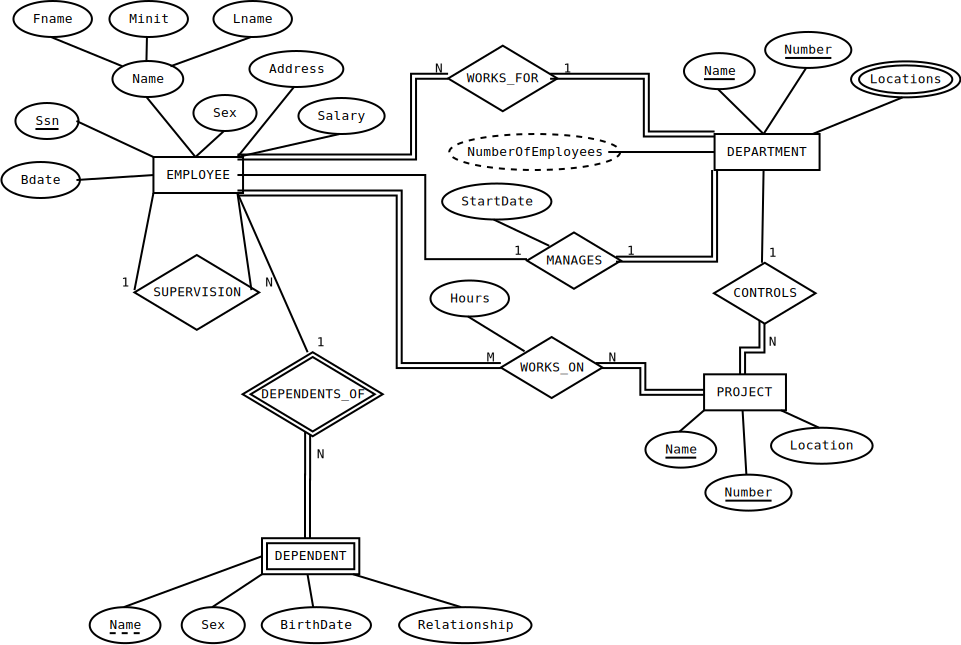
\includegraphics[width=0.6\textwidth]{exemplos/diagramas/ER.jpeg}
    \fonte{Indicar autor original.}
\end{figure}


\begin{figure}
    \centering
    \caption{Exemplo de diagrama - salvo imagem vetorizada - EPS}
    \label{fig:uml_dia_vetorizado_eps}
	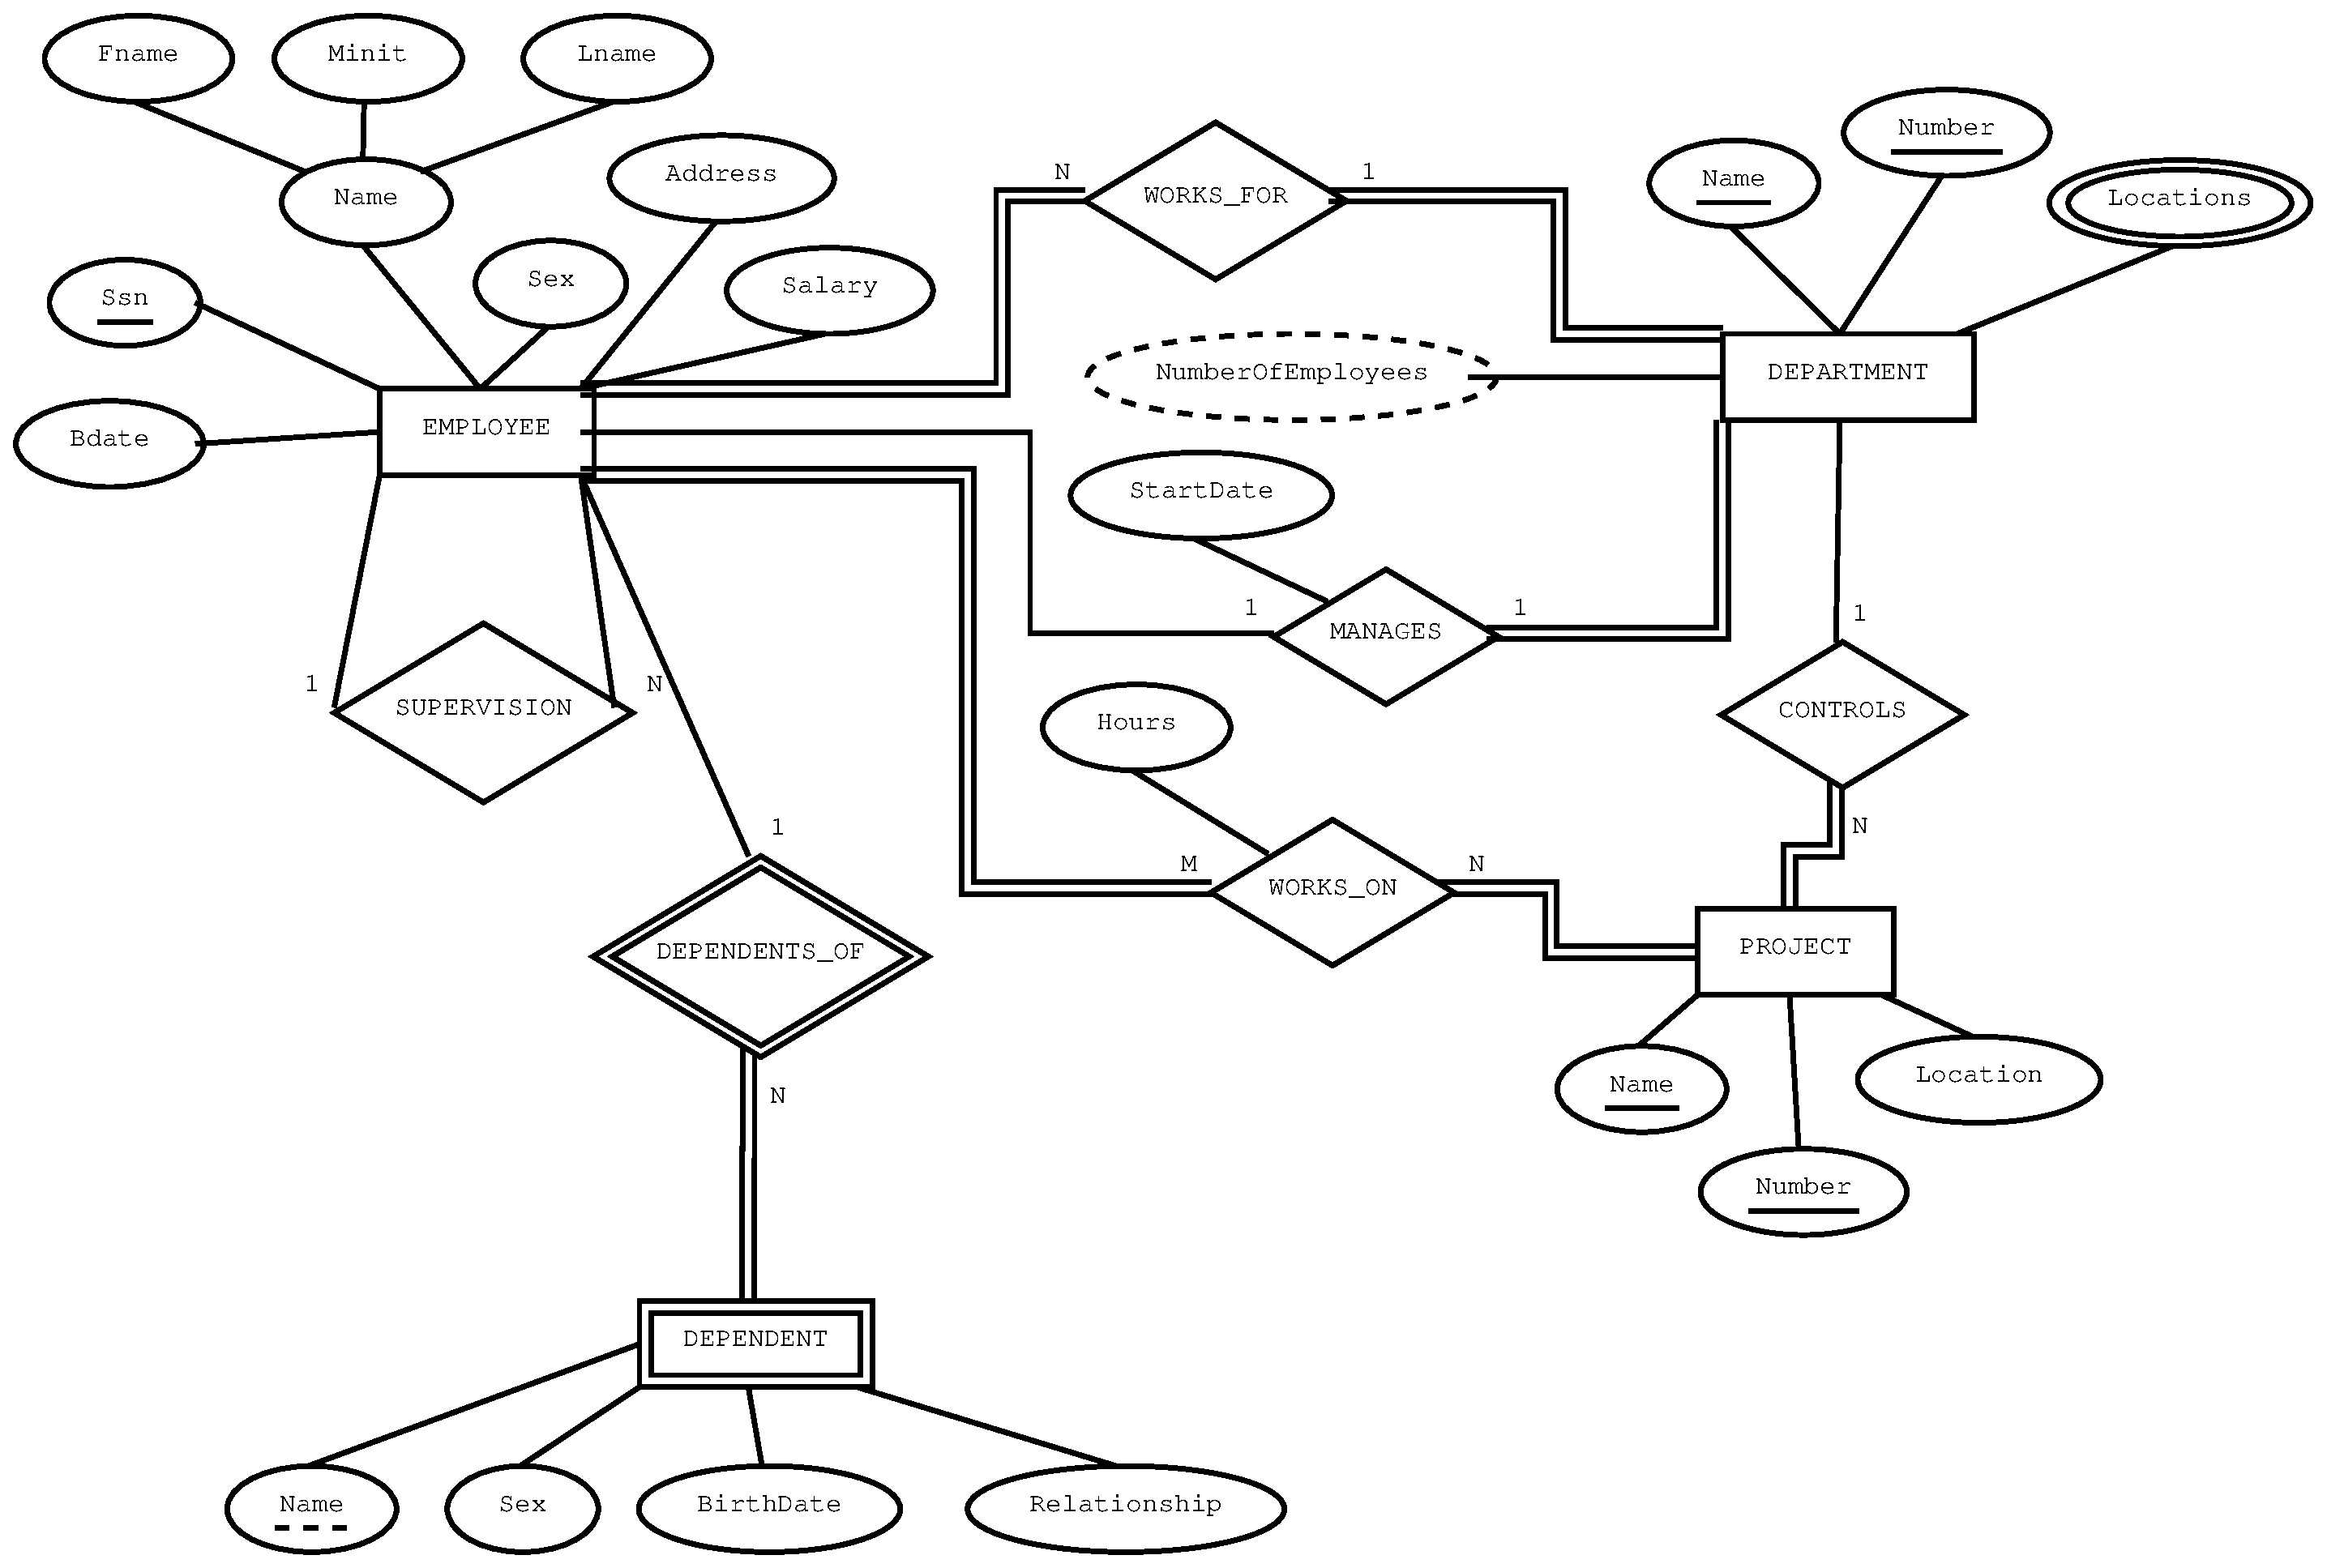
\includegraphics[width=0.6\textwidth]{exemplos/diagramas/ER.eps}
    \fonte{Indicar autor original.}
\end{figure}

\begin{figure}
    \centering
    \caption{Exemplo de diagrama - salvo imagem vetorizada - SVG}
    \label{fig:uml_dia_vetorizado_svg}
    \includesvg[inkscapelatex=false,width=0.6\textwidth]{exemplos/diagramas/ER.svg}
    \fonte{Indicar autor original.}
\end{figure}



% generated by Plantuml 7997beta
\definecolor{plantucolor0000}{RGB}{254,254,206}
\definecolor{plantucolor0001}{RGB}{168,0,54}
\definecolor{plantucolor0002}{RGB}{173,209,178}
\definecolor{plantucolor0003}{RGB}{0,0,0}
\definecolor{plantucolor0004}{RGB}{0,0,255}

\begin{figure}[htb]
    \centering
    \caption{\label{diagramauml}Exemplo de Diagrama UML gerado a partir do PlantUML}
\begin{tikzpicture}[yscale=-1]
\draw[color=plantucolor0001,fill=plantucolor0000,line width=1.5pt] (131pt,29pt) rectangle (223pt,90.8359pt);
\draw[color=plantucolor0001,fill=plantucolor0002,line width=1.0pt] (146pt,45pt) ellipse (11pt and 11pt);
\draw[color=black,fill=black] (148.7656pt,40.875pt) ..controls (148.9219pt,40.6563pt) .. (149.1094pt,40.5469pt) ..controls (149.2969pt,40.4375pt) .. (149.5156pt,40.4375pt) ..controls (149.8906pt,40.4375pt) .. (150.125pt,40.6953pt) ..controls (150.3594pt,40.9531pt) .. (150.3594pt,41.5625pt) -- (150.3594pt,43.0156pt) ..controls (150.3594pt,43.625pt) .. (150.125pt,43.8906pt) ..controls (149.8906pt,44.1563pt) .. (149.5156pt,44.1563pt) ..controls (149.1719pt,44.1563pt) .. (148.9688pt,43.9531pt) ..controls (148.7656pt,43.7656pt) .. (148.6563pt,43.25pt) ..controls (148.6094pt,42.8906pt) .. (148.4219pt,42.7031pt) ..controls (148.0938pt,42.3281pt) .. (147.4844pt,42.1094pt) ..controls (146.875pt,41.8906pt) .. (146.25pt,41.8906pt) ..controls (145.4844pt,41.8906pt) .. (144.8516pt,42.2188pt) ..controls (144.2188pt,42.5469pt) .. (143.7266pt,43.2969pt) ..controls (143.2344pt,44.0469pt) .. (143.2344pt,45.0781pt) -- (143.2344pt,46.1719pt) ..controls (143.2344pt,47.4063pt) .. (144.125pt,48.2266pt) ..controls (145.0156pt,49.0469pt) .. (146.6094pt,49.0469pt) ..controls (147.5469pt,49.0469pt) .. (148.2031pt,48.7969pt) ..controls (148.5938pt,48.6406pt) .. (149.0156pt,48.2031pt) ..controls (149.2813pt,47.9375pt) .. (149.4297pt,47.8594pt) ..controls (149.5781pt,47.7813pt) .. (149.7813pt,47.7813pt) ..controls (150.1094pt,47.7813pt) .. (150.3672pt,48.0391pt) ..controls (150.625pt,48.2969pt) .. (150.625pt,48.6406pt) ..controls (150.625pt,48.9844pt) .. (150.2813pt,49.3906pt) ..controls (149.7813pt,49.9688pt) .. (148.9844pt,50.2969pt) ..controls (147.9063pt,50.75pt) .. (146.6094pt,50.75pt) ..controls (145.0938pt,50.75pt) .. (143.8906pt,50.125pt) ..controls (142.9063pt,49.625pt) .. (142.2188pt,48.5547pt) ..controls (141.5313pt,47.4844pt) .. (141.5313pt,46.2031pt) -- (141.5313pt,45.0469pt) ..controls (141.5313pt,43.7188pt) .. (142.1484pt,42.5703pt) ..controls (142.7656pt,41.4219pt) .. (143.8594pt,40.8047pt) ..controls (144.9531pt,40.1875pt) .. (146.1875pt,40.1875pt) ..controls (146.9219pt,40.1875pt) .. (147.5703pt,40.3516pt) ..controls (148.2188pt,40.5156pt) .. (148.7656pt,40.875pt);
\node at (160pt,37.4531pt)[below right]{Subscriber};
\draw[color=plantucolor0001,line width=1.5pt] (132pt,61pt) -- (222pt,61pt);
\node at (137pt,65pt)[below right]{subscriberId};
\draw[color=plantucolor0001,line width=1.5pt] (132pt,82.8359pt) -- (222pt,82.8359pt);
\draw[color=plantucolor0001,fill=plantucolor0000,line width=1.5pt] (31pt,212pt) rectangle (137pt,273.8359pt);
\draw[color=plantucolor0001,fill=plantucolor0002,line width=1.0pt] (46pt,228pt) ellipse (11pt and 11pt);
\draw[color=black,fill=black] (48.7656pt,223.875pt) ..controls (48.9219pt,223.6563pt) .. (49.1094pt,223.5469pt) ..controls (49.2969pt,223.4375pt) .. (49.5156pt,223.4375pt) ..controls (49.8906pt,223.4375pt) .. (50.125pt,223.6953pt) ..controls (50.3594pt,223.9531pt) .. (50.3594pt,224.5625pt) -- (50.3594pt,226.0156pt) ..controls (50.3594pt,226.625pt) .. (50.125pt,226.8906pt) ..controls (49.8906pt,227.1563pt) .. (49.5156pt,227.1563pt) ..controls (49.1719pt,227.1563pt) .. (48.9688pt,226.9531pt) ..controls (48.7656pt,226.7656pt) .. (48.6563pt,226.25pt) ..controls (48.6094pt,225.8906pt) .. (48.4219pt,225.7031pt) ..controls (48.0938pt,225.3281pt) .. (47.4844pt,225.1094pt) ..controls (46.875pt,224.8906pt) .. (46.25pt,224.8906pt) ..controls (45.4844pt,224.8906pt) .. (44.8516pt,225.2188pt) ..controls (44.2188pt,225.5469pt) .. (43.7266pt,226.2969pt) ..controls (43.2344pt,227.0469pt) .. (43.2344pt,228.0781pt) -- (43.2344pt,229.1719pt) ..controls (43.2344pt,230.4063pt) .. (44.125pt,231.2266pt) ..controls (45.0156pt,232.0469pt) .. (46.6094pt,232.0469pt) ..controls (47.5469pt,232.0469pt) .. (48.2031pt,231.7969pt) ..controls (48.5938pt,231.6406pt) .. (49.0156pt,231.2031pt) ..controls (49.2813pt,230.9375pt) .. (49.4297pt,230.8594pt) ..controls (49.5781pt,230.7813pt) .. (49.7813pt,230.7813pt) ..controls (50.1094pt,230.7813pt) .. (50.3672pt,231.0391pt) ..controls (50.625pt,231.2969pt) .. (50.625pt,231.6406pt) ..controls (50.625pt,231.9844pt) .. (50.2813pt,232.3906pt) ..controls (49.7813pt,232.9688pt) .. (48.9844pt,233.2969pt) ..controls (47.9063pt,233.75pt) .. (46.6094pt,233.75pt) ..controls (45.0938pt,233.75pt) .. (43.8906pt,233.125pt) ..controls (42.9063pt,232.625pt) .. (42.2188pt,231.5547pt) ..controls (41.5313pt,230.4844pt) .. (41.5313pt,229.2031pt) -- (41.5313pt,228.0469pt) ..controls (41.5313pt,226.7188pt) .. (42.1484pt,225.5703pt) ..controls (42.7656pt,224.4219pt) .. (43.8594pt,223.8047pt) ..controls (44.9531pt,223.1875pt) .. (46.1875pt,223.1875pt) ..controls (46.9219pt,223.1875pt) .. (47.5703pt,223.3516pt) ..controls (48.2188pt,223.5156pt) .. (48.7656pt,223.875pt);
\node at (60pt,220.4531pt)[below right]{AccumUsage};
\draw[color=plantucolor0001,line width=1.5pt] (32pt,244pt) -- (136pt,244pt);
\node at (37pt,248pt)[below right]{subscriberId};
\draw[color=plantucolor0001,line width=1.5pt] (32pt,265.8359pt) -- (136pt,265.8359pt);
\draw[color=plantucolor0001,fill=plantucolor0000,line width=1.5pt] (221pt,191pt) rectangle (318pt,294.3438pt);
\draw[color=plantucolor0001,fill=plantucolor0002,line width=1.0pt] (240.05pt,207pt) ellipse (11pt and 11pt);
\draw[color=black,fill=black] (242.8156pt,202.875pt) ..controls (242.9719pt,202.6563pt) .. (243.1594pt,202.5469pt) ..controls (243.3469pt,202.4375pt) .. (243.5656pt,202.4375pt) ..controls (243.9406pt,202.4375pt) .. (244.175pt,202.6953pt) ..controls (244.4094pt,202.9531pt) .. (244.4094pt,203.5625pt) -- (244.4094pt,205.0156pt) ..controls (244.4094pt,205.625pt) .. (244.175pt,205.8906pt) ..controls (243.9406pt,206.1563pt) .. (243.5656pt,206.1563pt) ..controls (243.2219pt,206.1563pt) .. (243.0188pt,205.9531pt) ..controls (242.8156pt,205.7656pt) .. (242.7063pt,205.25pt) ..controls (242.6594pt,204.8906pt) .. (242.4719pt,204.7031pt) ..controls (242.1438pt,204.3281pt) .. (241.5344pt,204.1094pt) ..controls (240.925pt,203.8906pt) .. (240.3pt,203.8906pt) ..controls (239.5344pt,203.8906pt) .. (238.9016pt,204.2188pt) ..controls (238.2688pt,204.5469pt) .. (237.7766pt,205.2969pt) ..controls (237.2844pt,206.0469pt) .. (237.2844pt,207.0781pt) -- (237.2844pt,208.1719pt) ..controls (237.2844pt,209.4063pt) .. (238.175pt,210.2266pt) ..controls (239.0656pt,211.0469pt) .. (240.6594pt,211.0469pt) ..controls (241.5969pt,211.0469pt) .. (242.2531pt,210.7969pt) ..controls (242.6438pt,210.6406pt) .. (243.0656pt,210.2031pt) ..controls (243.3313pt,209.9375pt) .. (243.4797pt,209.8594pt) ..controls (243.6281pt,209.7813pt) .. (243.8313pt,209.7813pt) ..controls (244.1594pt,209.7813pt) .. (244.4172pt,210.0391pt) ..controls (244.675pt,210.2969pt) .. (244.675pt,210.6406pt) ..controls (244.675pt,210.9844pt) .. (244.3313pt,211.3906pt) ..controls (243.8313pt,211.9688pt) .. (243.0344pt,212.2969pt) ..controls (241.9563pt,212.75pt) .. (240.6594pt,212.75pt) ..controls (239.1438pt,212.75pt) .. (237.9406pt,212.125pt) ..controls (236.9563pt,211.625pt) .. (236.2688pt,210.5547pt) ..controls (235.5813pt,209.4844pt) .. (235.5813pt,208.2031pt) -- (235.5813pt,207.0469pt) ..controls (235.5813pt,205.7188pt) .. (236.1984pt,204.5703pt) ..controls (236.8156pt,203.4219pt) .. (237.9094pt,202.8047pt) ..controls (239.0031pt,202.1875pt) .. (240.2375pt,202.1875pt) ..controls (240.9719pt,202.1875pt) .. (241.6203pt,202.3516pt) ..controls (242.2688pt,202.5156pt) .. (242.8156pt,202.875pt);
\node at (254.95pt,199.4531pt)[below right]{IpSession};
\draw[color=plantucolor0001,line width=1.5pt] (222pt,223pt) -- (317pt,223pt);
\node at (227pt,227pt)[below right]{ipAddress};
\node at (227pt,240.8359pt)[below right]{specificData};
\node at (227pt,254.6719pt)[below right]{sapcOriginStateId};
\node at (227pt,268.5078pt)[below right]{apnId};
\draw[color=plantucolor0001,line width=1.5pt] (222pt,286.3438pt) -- (317pt,286.3438pt);
\draw[color=plantucolor0004] (191.942pt,90.081pt) ..controls (205.204pt,115.893pt) and (224.952pt,154.325pt) .. (241.265pt,186.076pt);
\draw[color=plantucolor0004,fill=plantucolor0004] (243.646pt,190.709pt) -- (243.0894pt,180.8759pt) -- (241.3604pt,186.262pt) -- (235.9742pt,184.5329pt) -- (243.646pt,190.709pt) -- cycle;
\node at (191.0584pt,98.9168pt)[below right]{1};
\node at (230.3817pt,166.6703pt)[below right]{1..*};
\draw[color=plantucolor0001] (162.058pt,90.081pt) ..controls (145.645pt,122.023pt) and (119.302pt,173.295pt) .. (101.824pt,207.31pt);
\draw[color=plantucolor0001,fill=plantucolor0001] (99.5252pt,211.784pt) -- (107.1969pt,205.6078pt) -- (101.8108pt,207.337pt) -- (100.0816pt,201.9509pt) -- (99.5252pt,211.784pt) -- cycle;
\node at (143.0082pt,98.7264pt)[below right]{1};
\node at (101.801pt,187.522pt)[below right]{0..1};
\end{tikzpicture}
	\legend{Fonte: Exemplos PlantUML.}
\end{figure}

A \autoref{fig_diag_virado} exemplifica como utilizar uma imagem em formato paisagem (página inteira). Obs: Utilizamos propositalmente uma imagem não vetorizada de forma a ilustrar o procedimento e também para apresentar que a qualidade não fica boa o suficiente para leitura. Uma versão vetorizada dessa figura teria qualidade melhor.


% observe que a imagem a seguir teve que ser ajustada para caber corretamente na página
% por não ser uma imagem vetorizada a qualidade não é a melhor possivel
\begin{sidewaysfigure}[htb]
    \centering
	\caption{\label{fig_diag_virado}Diagrama Virado - Exemplo}
	\includegraphics[width=0.9\textwidth]{exemplos/exemplo_diag_horizontal.png}
	\fonte{\citeonline{openehrCompositionEntry}.}
\end{sidewaysfigure}


\subsection{Impressão em folhas formato A3}

A página seguinte em A3 permite a impressão de diagramas grandes que não podem ser visualizados facilmente em folha padrão A4. Lembre que algumas impressoras podem ter problemas com isso, então selecione somente as páginas A4 ao imprimir e depois imprima separadamente a página A3.

A \autoref{fig_logo_A3} utiliza a mesma imagem da \autoref{fig_logo} e foi ampliada para demonstrar a essa possibilidade de impressão de grandes imagens em A3.

Observe que o código de exemplo vai gerar uma quebra de página no local onde for definida a página A3, por isso não deve ser utilizado entre textos para evitar grandes espaços em branco.

Folhas impressas em A3 ou tamanhos maiores devem ser dobradas seguindo o padrão definido pela ABNT. 


Cuidado ao utilizar folhas A3 em um documento impresso em frente e verso pois a numeração das páginas seguintes pode ser impressa de forma incorreta (posição do número na página). Uma alternativa para esta situação é manter todas páginas impressas em A3 no último apêndice, fazendo as referencias corretas durante o texto.



\afterpage{%
\begin{PAGINA-A3}

\begin{figure}[p]
    \centering%
    \fcolorbox{red}{yellow}{ \includegraphics[height=\textheight,width=\textwidth,keepaspectratio]{\ifspprefixo/logo-02.jpg}}%
	\caption{\label{fig_logo_A3}Logotipo IFSP em página A3}
	\legend{Com borda para demonstrar os limites}
   \fonte{Autor da Figura}
\end{figure}

\end{PAGINA-A3}
}





% ---
% Conclusão (outro exemplo de capítulo sem numeração e presente no sumário)
% Dependendo do trabalho desenvolvido ele pode ter uma Conclusão ou Considerações finais
% Para trabalhos de disciplina utilizar Considerações Finais
% ---
\chapter{Considerações Finais}
% Exemplo de como adicionar linha adicional no sumário
Com a matéria de Projeto Integrado I (PI1A5), foi possível vivenciar, de fato, as etapas e desafios que envolvem desenvolver um software e sua documentação.

A experiência de realizar o projeto envolveu, acima de tudo, dificuldades diversas às quais foram necessárias adaptações, fossem elas individuais ou da equipe inteira. Todas essas dificuldades foram de extremo valor, já que puderam mostrar o quão importante são alguns fatores como: comunicação, sinceridade, atenção e proatividade.

Como maiores pontos de dificuldade pelos quais a equipe passou, pode-se citar o conhecimento sobre o tema escolhido, conhecimento técnico sobre as ferramentas de desenvolvimento, gestão de tempo e informações sobre as requisições de cada entrega e, por fim, a documentação LaTeX. Para todos esses pontos de falha foi crucial que houvessem reuniões, alinhamentos e divisão de tarefas balanceadamente, para que não houvesse prejuízo para nenhuma das partes.

Foi preciso esforço de todos os membros da equipe para se informarem acerca do tema escolhido, a neurodiversidade, para que, dessa forma, fossem evitados equívocos de terminologias utilizadas e falta de fontes de informação sobre como é a rotina das pessoas neurodiversas. Quanto aos outros pontos de dificuldade pontuados, foram realizadas diversas reuniões e conversas informais para disseminação de conhecimento entre os membros, para que, o quanto antes, todos estivessem alinhados sobre todos os pontos do projeto.

Ao fim do projeto foi possível perceber a evolução de todos os envolvidos, tanto em âmbitos técnicos (hardskills) quanto em âmbitos comportamentais (softskills), além de ser possível perceber o quão mais entrosada a equipe estava.



% ----------------------------------------------------------
% Finaliza a parte no bookmark do PDF
% para que se inicie o bookmark na raiz
% e adiciona espaço de parte no Sumário
% ----------------------------------------------------------
\phantompart

% ----------------------------------------------------------
% ELEMENTOS PÓS-TEXTUAIS
% ----------------------------------------------------------
\postextual
% ----------------------------------------------------------

% ----------------------------------------------------------
% Referências bibliográficas
% ----------------------------------------------------------
\bibliography{referencias,exemplos/abntex2-doc-abnt-6023}

% ----------------------------------------------------------
% Glossário
% ----------------------------------------------------------
%
%
\ifdef{\printnoidxglossary}{
    \addcontentsline{toc}{chapter}{GLOSSÁRIO}
    \printnoidxglossary[style=glossario]
    %\printglossaries
}{}

% ----------------------------------------------------------
% Apêndices
% Documentos gerados pelo próprio autor
% ----------------------------------------------------------

% ---
% Inicia os apêndices
% ---
\begin{apendicesenv}

% Imprime uma página indicando o início dos apêndices
\partapendices

% ----------------------------------------------------------
\chapter{Quisque libero justo}
% ----------------------------------------------------------

\preencheComTexto

% ----------------------------------------------------------
\chapter{Nullam elementum urna vel imperdiet sodales elit ipsum pharetra ligula
ac pretium ante justo a nulla curabitur tristique arcu eu metus}
% ----------------------------------------------------------
\preencheComTexto

\end{apendicesenv}
% ---

% ----------------------------------------------------------
% Anexos
% Documentos gerados por outros autores
% ----------------------------------------------------------

% ---
% Inicia os anexos
% ---
\begin{anexosenv}
\anexos
% Imprime uma página indicando o início dos anexos
\partanexos

% ---
\chapter{Manual todonotes(parcial)}
\label{manual-todonotes}
% ---
\index{pdf}
% se pages = "-"  fica com arquivo completo
\includepdf[pages=1-3,scale=0.8,frame=true,pagecommand={}]{anexos/todonotes.pdf}

% ---
% Para incluir sem gerar a quebra de página inicial no anexo
\includepdf[pages=1,scale=0.7,frame=true,pagecommand=\chapter{Manual pdfpages(parcial)}\label{manual-pdfpages}]{anexos/pdfpages.pdf}
\includepdf[pages=2-3,scale=0.8,frame=true,pagecommand={}]{anexos/pdfpages.pdf}

% ---
\chapter{Manual acronym(parcial)}
\index{pdf}
% somente algumas páginas para exemplo sem borda
\includepdf[pages=1-3,frame=false,pagecommand={}]{anexos/acronym.pdf}



\includepdf[frame=true,scale=0.7,pagecommand=\chapter{Referência Rápida pifont}\label{pifont-quickref}]{anexos/pifont.pdf}


\end{anexosenv}



%---------------------------------------------------------------------
% INDICE REMISSIVO - Quando necessário 
% As palavras indexadas devem ser definidas com \index{} no texto
%---------------------------------------------------------------------
\phantompart
\printindex
\todonum[inline]{remover indice remissivo se não for necessário}

%---------------------------------------------------------------------

\end{document}